%%
%% This is file `sample.tex'
%%
%% ------------------------------------------------------------------------
%% Copyright (C) 2021,2022 Q.Tang
%% 
%% Licensed under the Apache License, Version 2.0 (the "License");
%% you may not use this file except in compliance with the License.
%% You may obtain a copy of the License at
%% 
%%     http://www.apache.org/licenses/LICENSE-2.0
%% 
%% Unless required by applicable law or agreed to in writing, software
%% distributed under the License is distributed on an "AS IS" BASIS,
%% WITHOUT WARRANTIES OR CONDITIONS OF ANY KIND, either express or implied.
%% See the License for the specific language governing permissions and
%% limitations under the License.
%% ------------------------------------------------------------------------

\documentclass[aspectratio=169,12pt]{beamer}             

\usetheme{bjtubeamer}
\graphicspath{{figures/}}
\usetikzlibrary{positioning}
\usetikzlibrary{arrows.meta}
\usepackage{varwidth}

\definecolor{gray}{HTML}{E7E6E6}
\definecolor{darkgray}{HTML}{7F7F7F}
\definecolor{yellow}{HTML}{F9C36B}
\definecolor{blue}{HTML}{9BC2E5}
\definecolor{captiongray}{HTML}{AFABAB}
\definecolor{darkred}{HTML}{BE0000}
\definecolor{darkgreen}{HTML}{538234}
\definecolor{darkblue}{HTML}{2E528E}

\renewcommand{\figurename}{} 
\DeclareCaptionLabelSeparator{twospace}{\ ~}
\captionsetup{labelsep=twospace}

\justifying\let\raggedright\justifying

\title{联合单目深度估计的深度图像超分辨率重建算法研究}
\englishtitle{Research on Joint Depth Map Super-Resolution and Monocular Depth Estimation Algorithm}
\author{唐麒}
\studentNumber{17301138}
\advisor{冯凤娟}
\institution{软件学院}
\defense{本科毕业设计答辩}
\begin{document}
\maketitle
\makecontent

\section{项目简介}

\subsection{项目来源}
\begin{frame}[t]
	\frametitle{项目来源}
	\vspace{0.3cm}
	\begin{tikzpicture}
		\useasboundingbox (0,0) rectangle(\the\paperwidth,\the\paperheight);
%		\draw[help lines] (0,0) grid (12,12);
		\draw[draw=none,fill=gray] (0.2,8.8) rectangle(11,4.8);
		\node[anchor=north east] at ({\the\paperwidth-2cm,\the\paperheight+1.8}) {\includegraphics[height=4.2cm]{0.jpeg}};
		\node[anchor=north east] at ({6.1cm,\the\paperheight-4.8cm}) {
\includegraphics[height=1cm]{1.png}};
		\node[anchor=north east] at ({\the\paperwidth-2cm,\the\paperheight-4.8cm}) {
\includegraphics[height=1cm]{2.png}};
		\node[anchor=north west, draw=none,align=left] at (0.3,8.65) {\footnotesize 联合单目深度估计的深度图\\\footnotesize 像超分辨率重建算法研究};
		\node[anchor=north west, draw=none,align=left] at (0.35,7.58) {\scriptsize 算法研究岗};
		\node[anchor=north west, draw=none,align=right] at (5.9,8.6) {\scriptsize \color{red}北京交通大学\\\scriptsize \color{red}信息科学研究所};
		\node[anchor=north west, draw=none,align=right] at (4.8,7.58) {\scriptsize 2020年10月29日- 至今};
		\node[anchor=north west, draw=none,align=left] at (0.35,7.05) {\scriptsize 探索深度图超分辨率重建任务中颜色引导、细节恢复、模态交\\\scriptsize 互等问题的解决方案。具体地,从多任务学习的角度出发研究\\\scriptsize 一种联合深度估计的深度图超分辨率网络,并探索两个任务之\\\scriptsize 间的交互指导关系,以达到相互促进、互利共赢的效果。
};
	\end{tikzpicture}
	
\end{frame}

\subsection{研究背景}
\begin{frame}[t]
	\vspace*{-.2cm}
	\begin{center}
		研究背景
	\end{center}
	
	\onslide<2->{
	\vspace{0.3cm}
    \begin{tikzpicture}
      	\draw[anchor=north west,draw=none,fill=blue,rounded corners=15pt] (4,-1) rectangle (6,0);
      	\node(node1p)[anchor=north west] at ({3.8cm,\the\paperheight-8.8cm}) {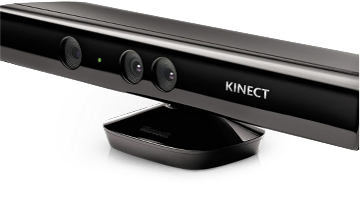
\includegraphics[height=1cm]{6.png}};
      	\node(node1t)[left = 1.5mm of node1p,shift={(0,0.5)},align=right]{1. 深度信息和深度相机};
      	\node[below = 0.2mm of node1t,align=right,font={\scriptsize}]{自动驾驶等依赖于高质量的深度信息\\[0.5em]便携式消费级深度相机的问世和普及};
      	\onslide<3->{
      		\draw[anchor=north west,draw=none,fill=yellow,rounded corners=15pt] (4,-3) rectangle (6,-4);
      		\node(node2p)[anchor=north west] at ({4.1cm,\the\paperheight-10.8cm}) {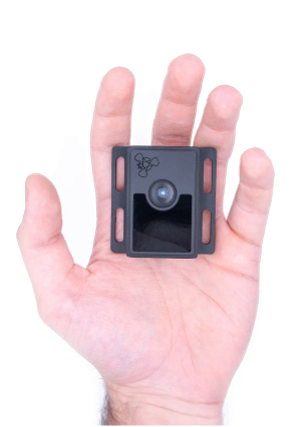
\includegraphics[height=2.2cm]{7.png}};
      		\node(node2t)[left = 1.5mm of node2p,shift={(0,0.3)},align=right]{2. 成像技术和图像分辨率};
      		\node[below = 0.2mm of node2t,align=right,font={\scriptsize}]{成像技术限制导致深度图像分辨率低\\[0.5em]硬件设施提高分辨率成本消耗较高等};
      	}
  		\onslide<4->{
  			\draw[anchor=north west,draw=none,fill=blue,rounded corners=15pt] (6.3,-3) rectangle (8.3,-4);
      		\node(node4p)[anchor=north west] at ({6.4cm,\the\paperheight-11.6cm}) {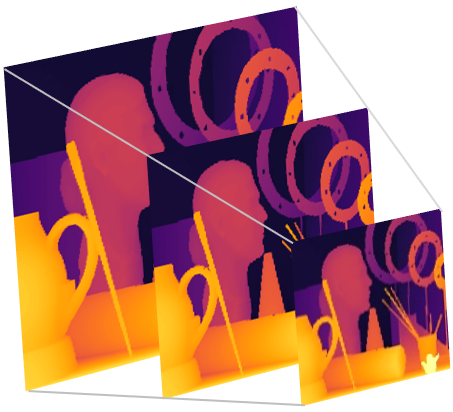
\includegraphics[height=1.5cm]{9.png}};
      		\node(node4t)[right = 1.5mm of node4p,shift={(0,0.7)},align=left]{3. 深度图像超分辨率重建};
      		\node[below = 0.2mm of node4t,align=left,font={\scriptsize}]{按照是否需要训练分为非学习式超分\\[0.5em]辨率重建算法和学习式超分辨率重建};
  		}
  		\onslide<5->{
        	\draw[anchor=north west,draw=none,fill=yellow,rounded corners=15pt] (6.3,-1) rectangle (8.3,0);
      		\node(node3p)[anchor=north west] at ({6.3cm,\the\paperheight-8.5cm}) {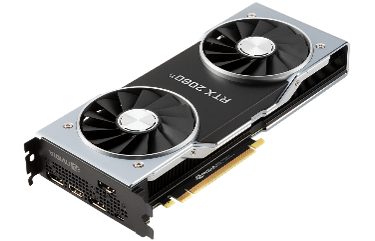
\includegraphics[height=1.3cm]{8.png}};
      		\node(node3t)[right = 0.5mm of node3p,shift={(-0.1,0.5)},align=left]{4. 深度学习};
      		\node[below = 0.2mm of node3t,shift={(1.3,0)},align=left,font={\scriptsize}]{自动驾驶等依赖于高质量的深度信息\\[0.5em]便携式消费级深度相机的问世和普及};
  
  		}
    \end{tikzpicture}
  }
\end{frame}

\subsection{研究意义}
\begin{frame}[t]
	\vspace*{-.2cm}
	\begin{center}
		研究意义	
	\end{center}
	\vspace{-.5cm}
	\begin{columns}
		\begin{column}{.30\linewidth}
			\begin{figure}
				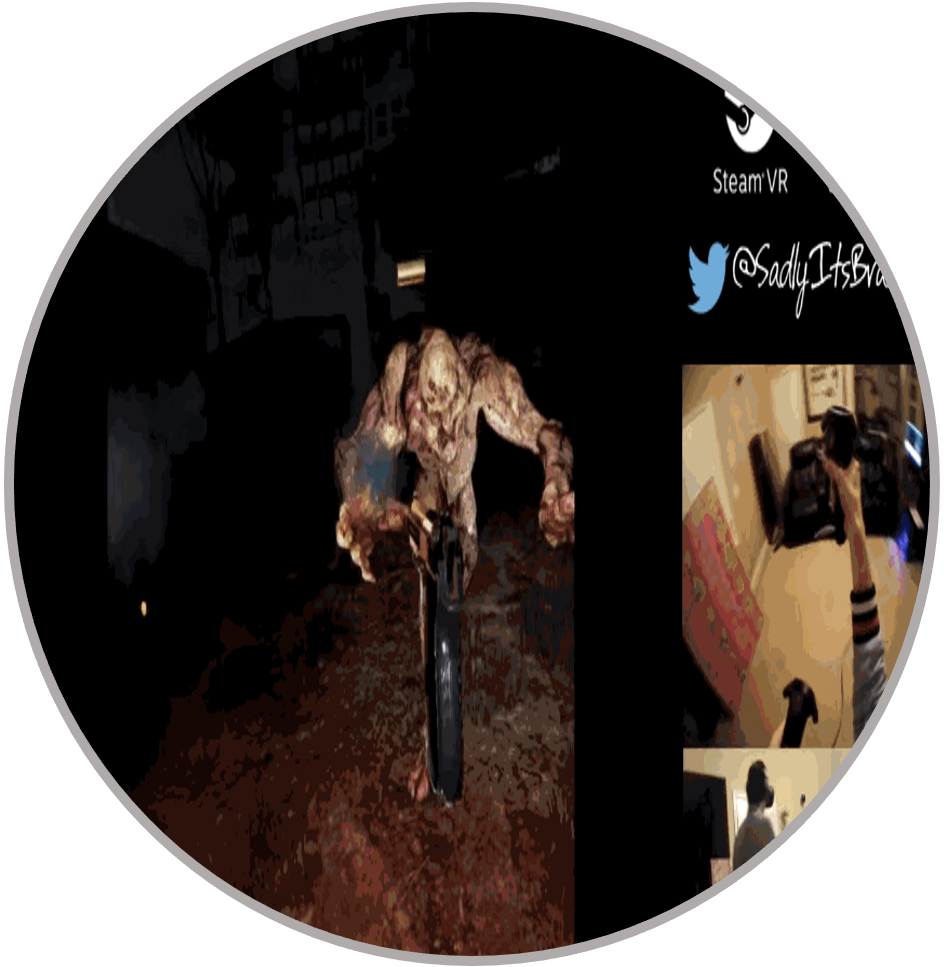
\includegraphics[height=3.5cm]{3.png}
			\end{figure}
			\begin{center}
				游戏领域\\[0.5em]
				{\small 获取玩家姿态动作\\
				可提高姿态识别率\\
				提升玩家游戏体验\\}
			\end{center}
		\end{column}
		\begin{column}{.30\linewidth}
			\begin{figure}
				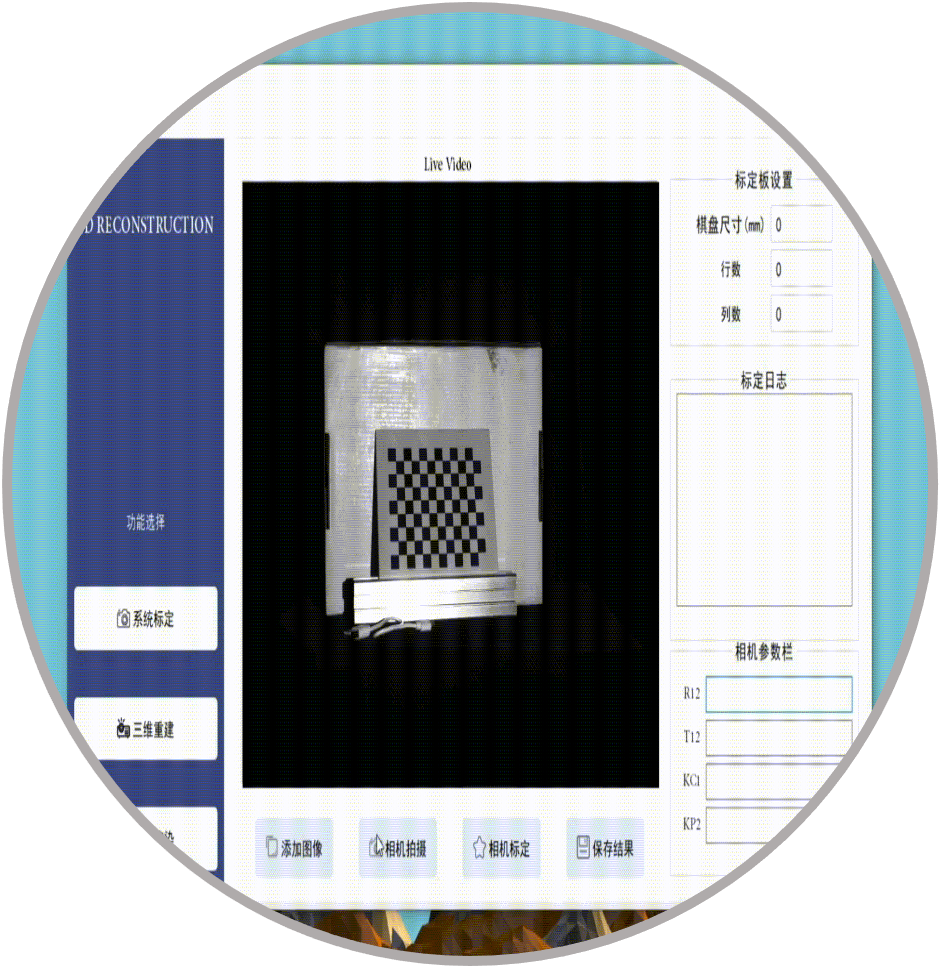
\includegraphics[height=3.5cm]{4.png}
			\end{figure}
			\begin{center}
				三维重建\\[0.5em]
				{\small 深度相机获取点云\\
				提高密集度和精度\\
				建模真实三维模型\\}
			\end{center}
		\end{column}
		\begin{column}{.30\linewidth}
			\begin{figure}
				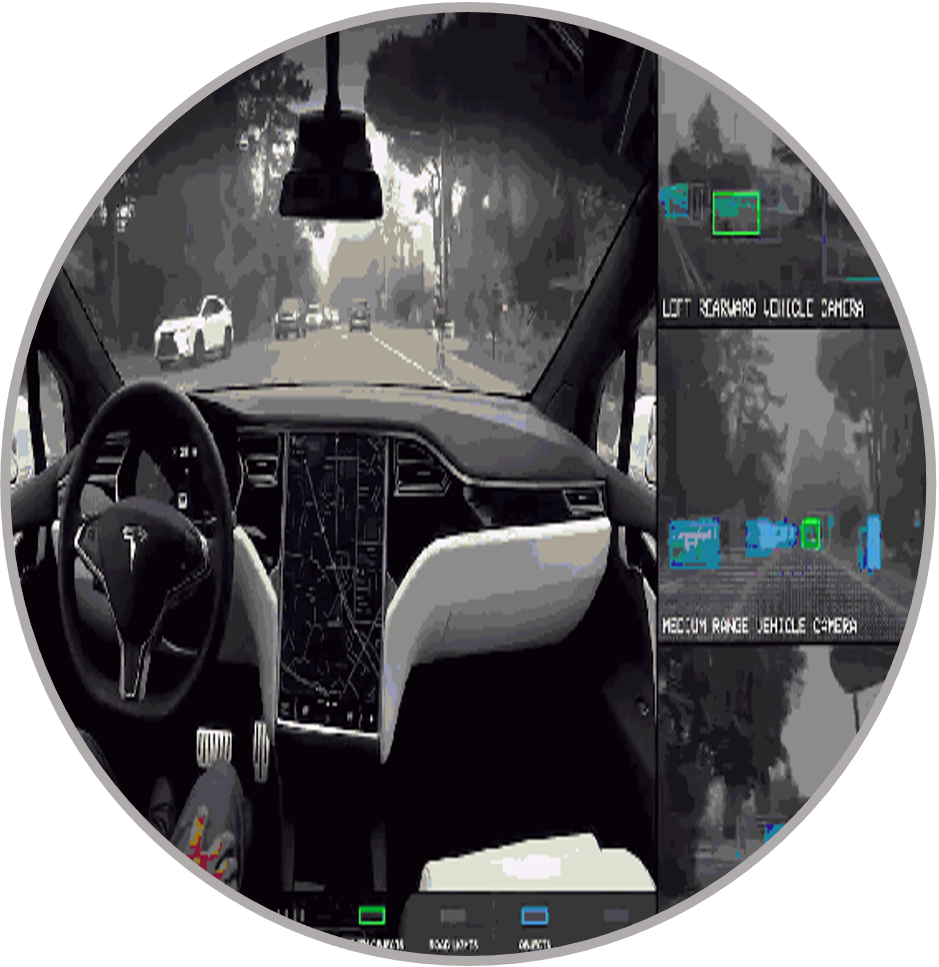
\includegraphics[height=3.5cm]{5.png}
			\end{figure}
			\begin{center}
				无人驾驶\\[0.5em]
				{\small 确定无人车辆位置\\
				获得更高定位精度\\
				环境描述/避障操作\\}
			\end{center}
		\end{column}
	\end{columns}
	
\end{frame}

\section{相关工作}
\subsection{项目目标}
\begin{frame}
	\frametitle{项目目标}
	\vspace{0.5cm}
	\begin{tikzpicture}
		\useasboundingbox (0,0) rectangle(\the\paperwidth,\the\paperheight);
		\draw[color=darkgray,dashed] (0,5)--(14,5);
		\draw[color=darkgray,dashed] (7,5.1)--(7,9);
		\node(p1)[anchor=north east] at({\the\paperwidth-9.5cm,\the\paperheight+0.1cm}) {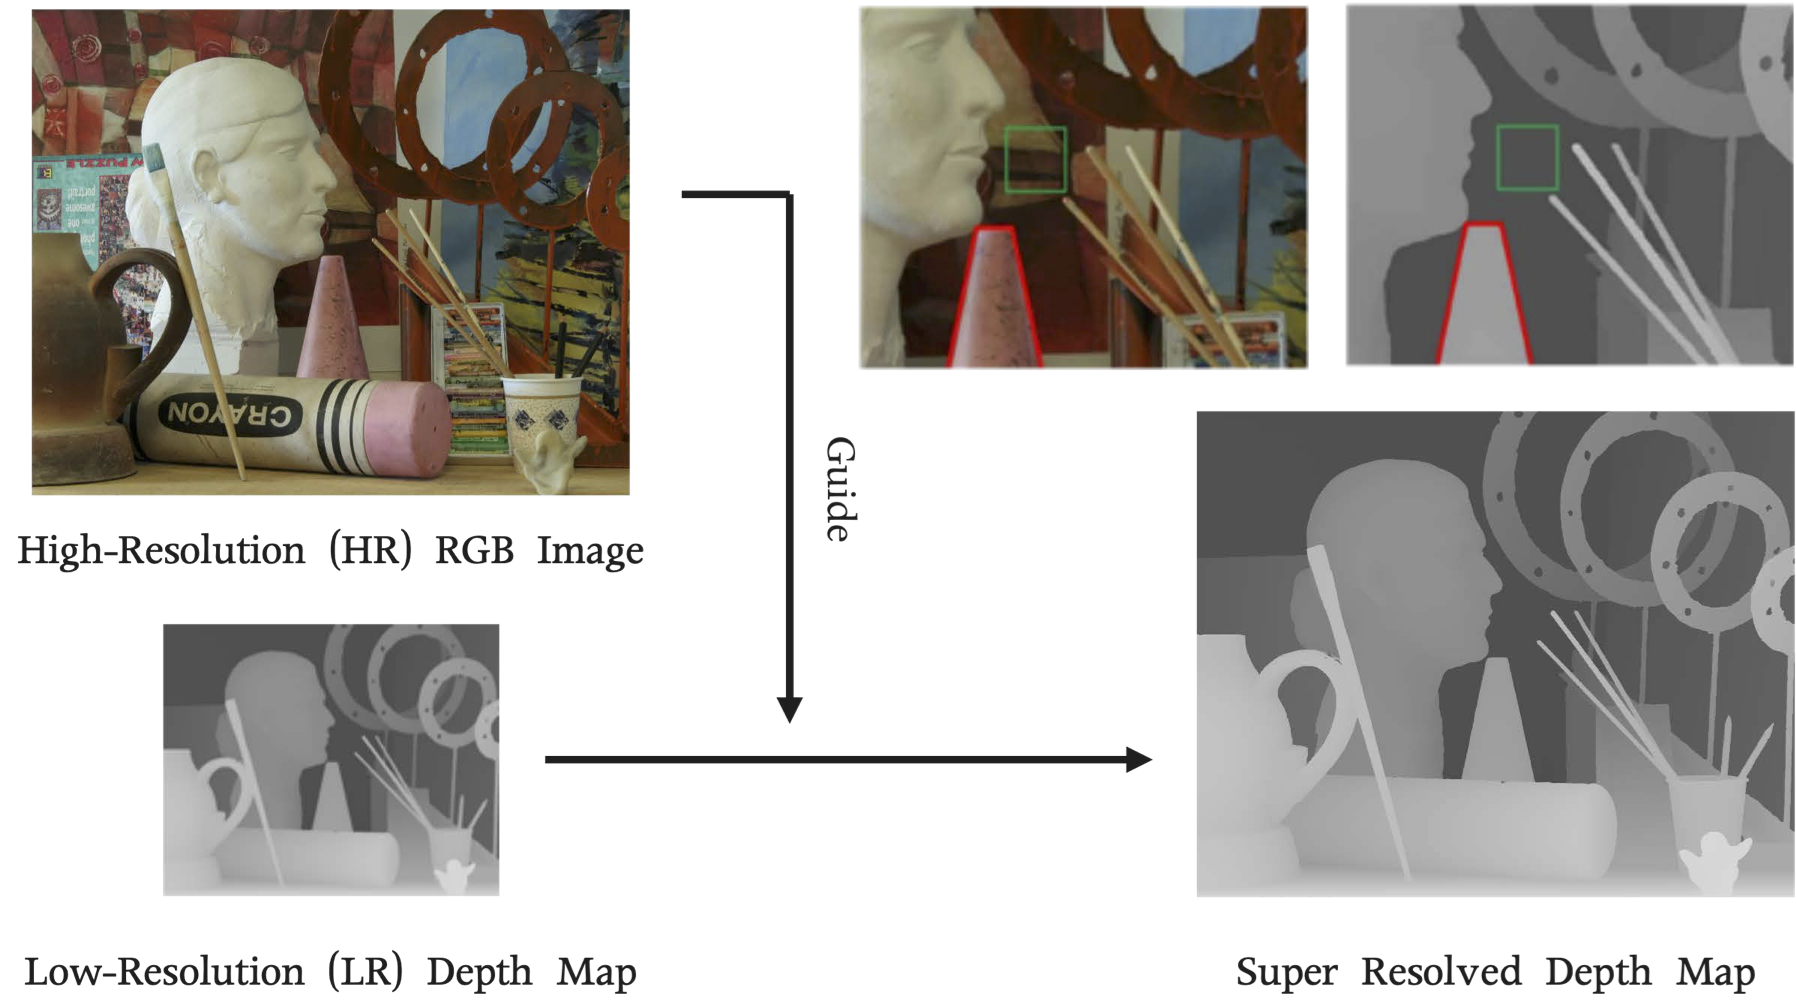
\includegraphics[scale=0.09]{10.png}};
		\node[below = 0.2mm of p1,align=center,font={\footnotesize}]{\color{red}(a) 深度图像超分辨率重建算法};
		
		\node(p2)[anchor=north east] at({\the\paperwidth-1.8cm,\the\paperheight-0.2cm}) {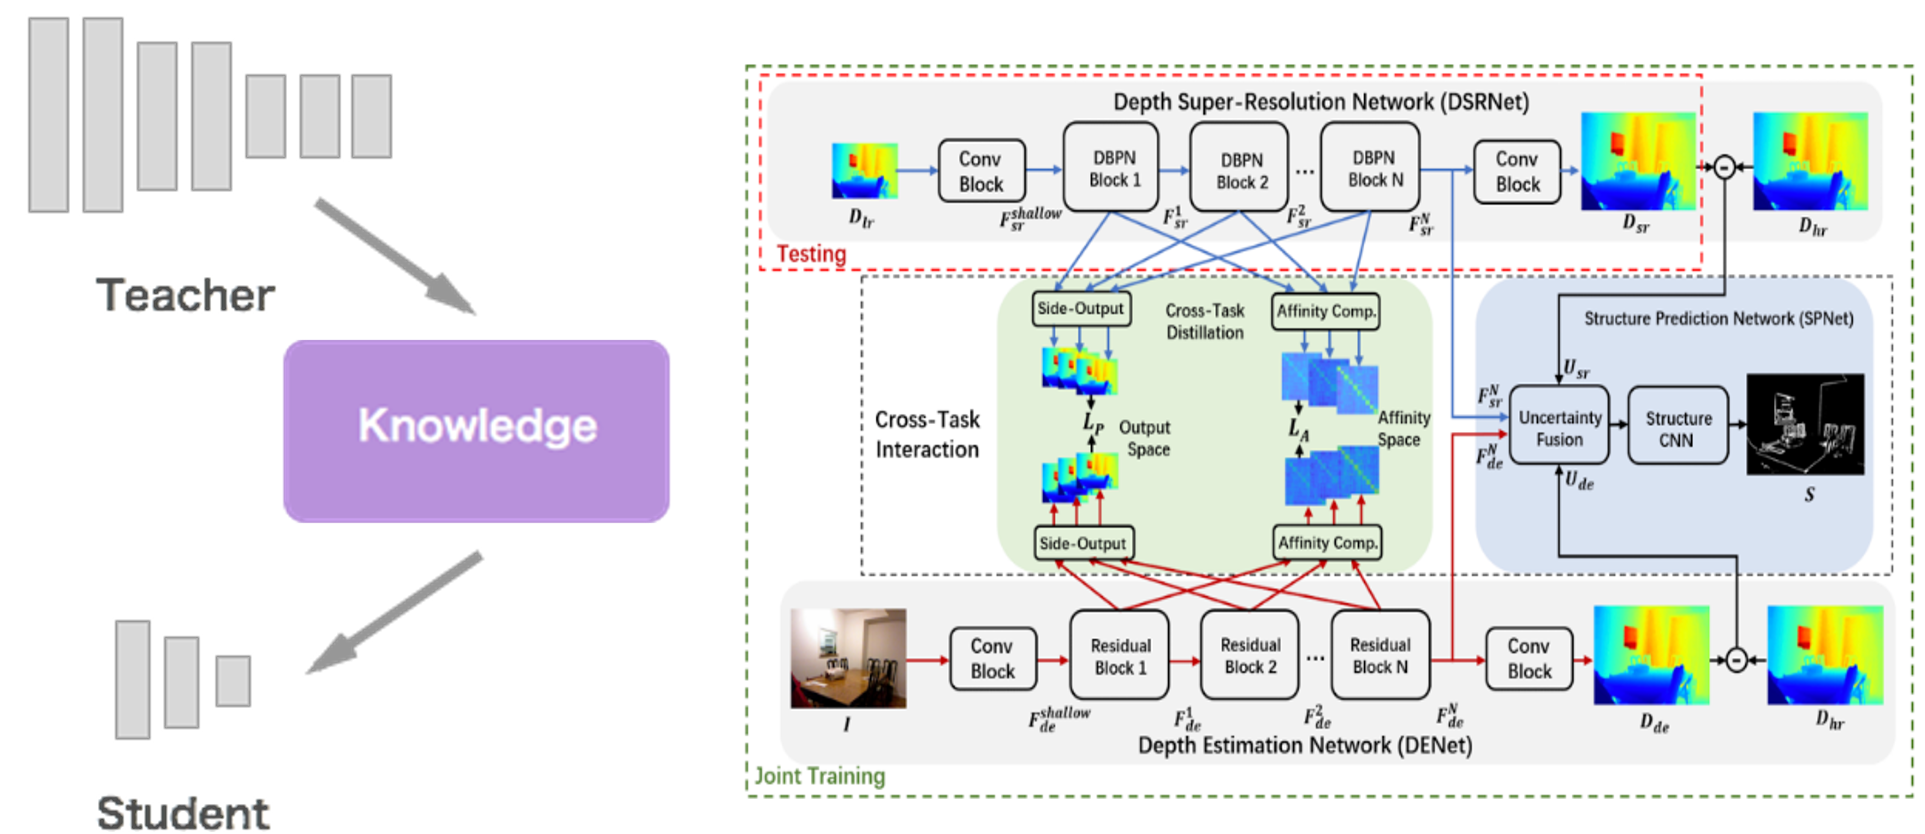
\includegraphics[scale=0.45]{11.png}};
		\node[below = 0.2mm of p2,align=center,font={\footnotesize}]{\color{red}(c) 面向深度图像的多任务联合学习};
		
		\node(p3)[anchor=north east] at({\the\paperwidth-2.7cm,\the\paperheight-4cm}) {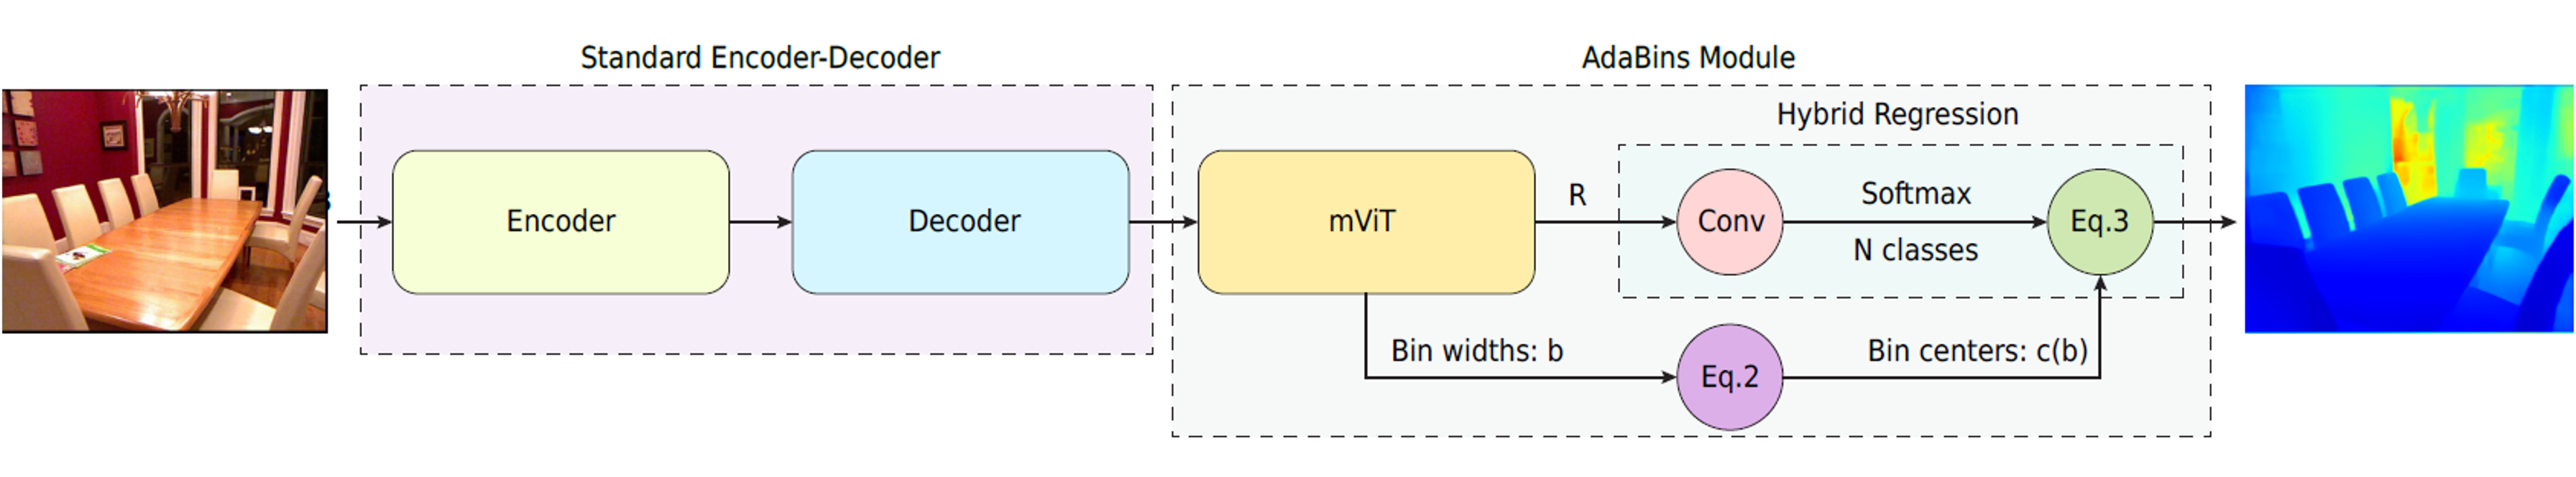
\includegraphics[scale=0.45]{12.png}};
		\node[below = 0.2mm of p3,align=center,shift={(-3,0.7cm)},font={\footnotesize}]{\color{red}(b) 单目深度估计};
		
		\node[anchor=north east,align=center,font={\small}] at (14,3.2) {\color{captiongray}图1 工作任务};

	\end{tikzpicture}

\end{frame}

\section{研究内容}
\subsection{网络设计}
\begin{frame}[t]
	\frametitle{BridgeNet}
%	\setcounter{figure}{2}
	\begin{columns}
		\begin{column}{.50\linewidth}
			\begin{figure}
				\centering
				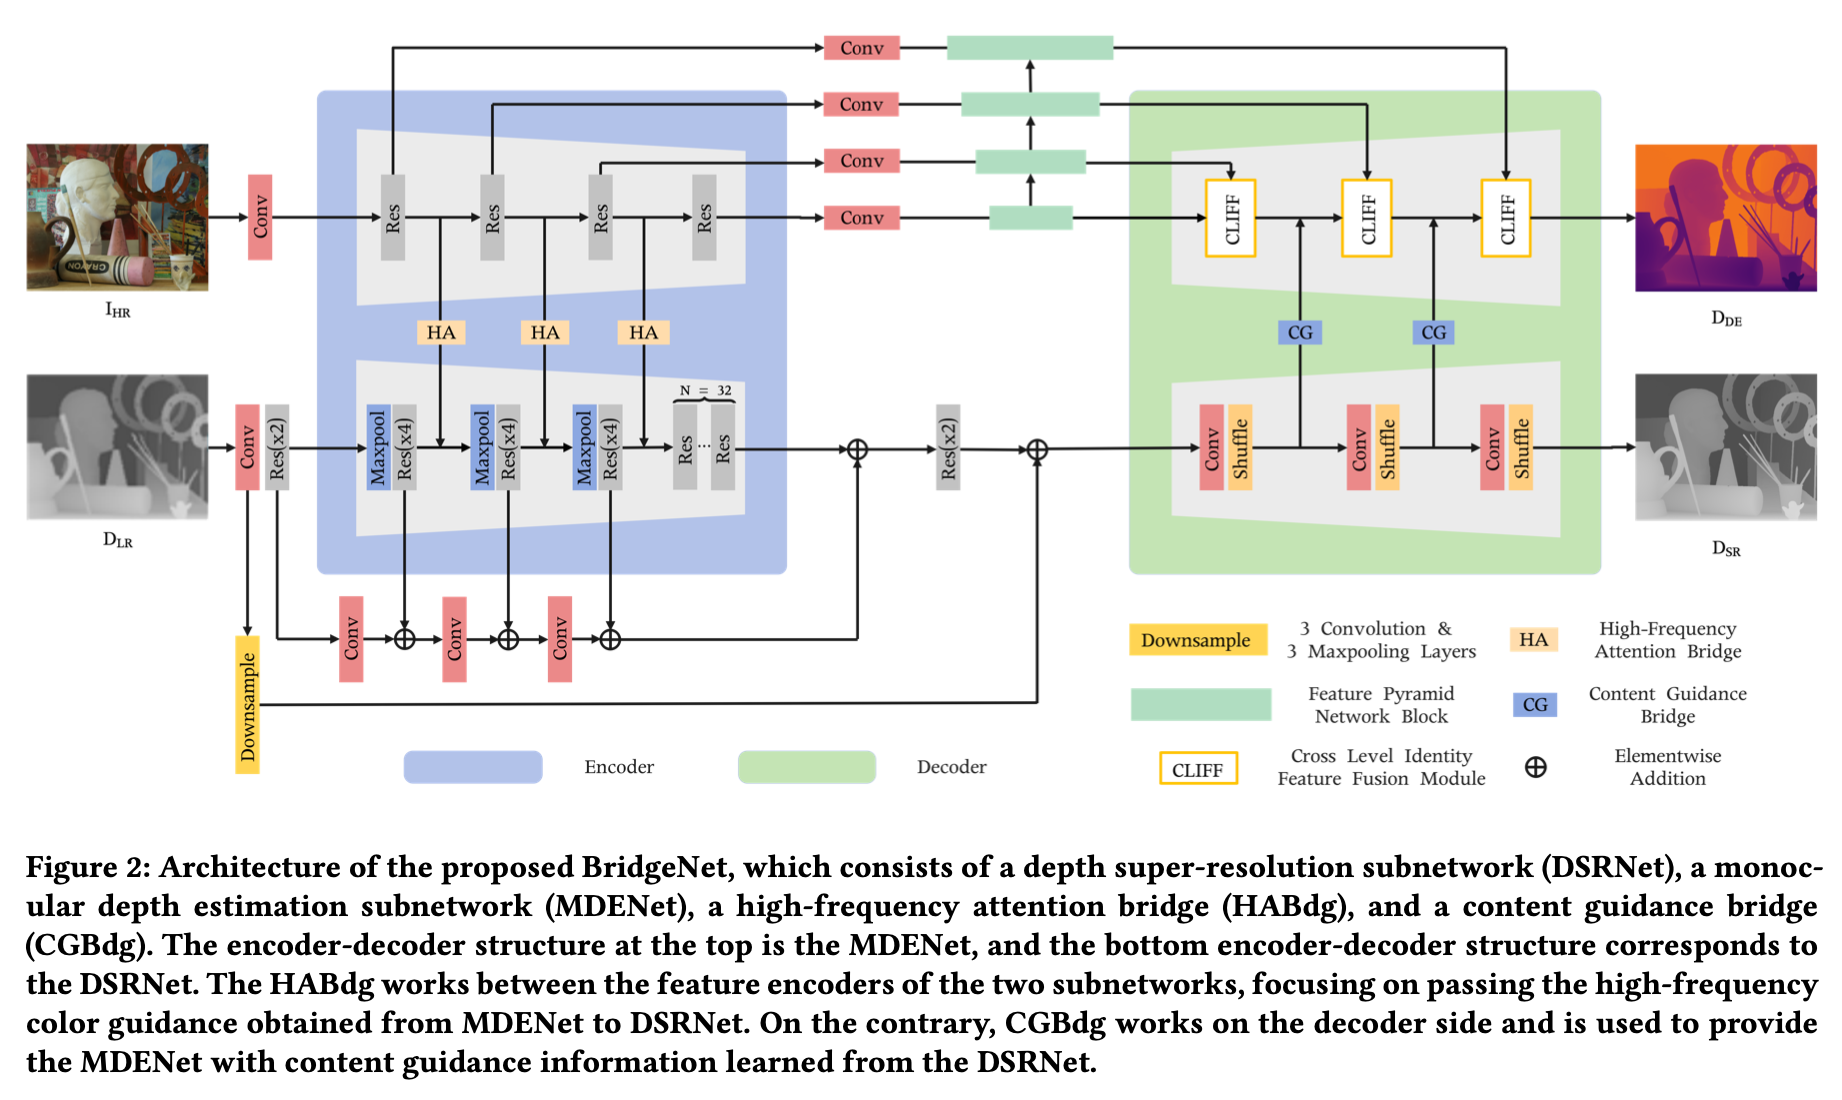
\includegraphics[scale=0.23]{13.png}
				\caption{\small \color{captiongray}图2 单目深度估计和深度图像超分辨率重建联合学习网络架构示意图}
			\end{figure}
		\end{column}
		\begin{column}{.50\linewidth}
			\begin{itemize}
			{\footnotesize
				\item 本文在{\color{red}联合学习网络}中将深度图像超分辨率重建任务和单目深度估计任务相关联,以提升深度图像超分辨率重建的性能。本文的整个网络结构具有高度的可移植性,可以为关联深度图像超分辨率重建和单目深度估计任务提供范例。
				\item 本文提出的联合学习网络包括深度图像超分辨率重建子网络(DSRNet)和单目深度估计子网络(MDENet),以及{\color{red}两个用于联合学习的桥接器},即高频注意力桥(HABdg)和内容引导桥(CGBdg)。
				\item 在不引入其他监督信息的情况下,本文的方法在多个公开基准数据集上均达到了{\color{red}具有竞争力的性能}。}
			\end{itemize}		
		\end{column}
	\end{columns}

\end{frame}

\begin{frame}[t]
	\frametitle{BridgeNet}
	\begin{columns}
		\begin{column}{.50\linewidth}
			\begin{figure}
				\centering
				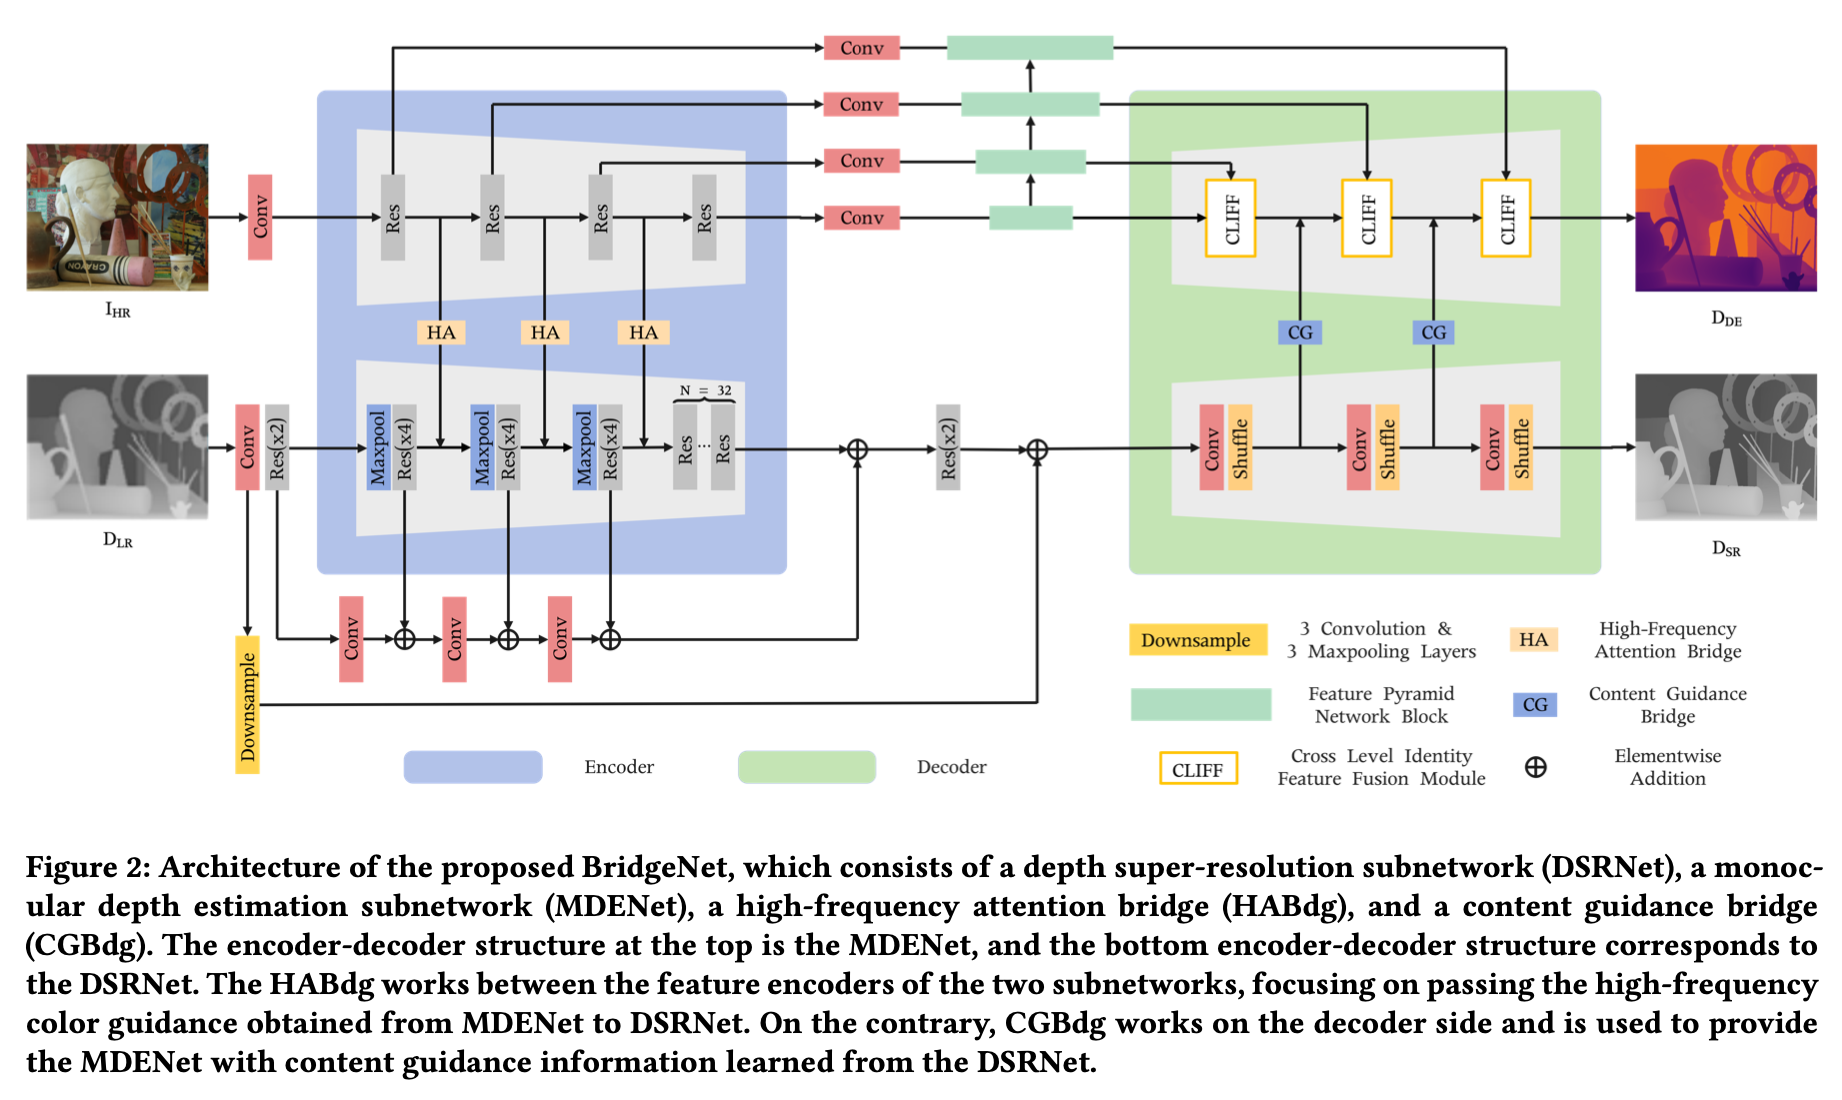
\includegraphics[scale=0.23]{13.png}
				\caption{\small \color{captiongray}图2 单目深度估计和深度图像超分辨率重建联合学习网络架构示意图}
			\end{figure}
		\end{column}
		\begin{column}{.50\linewidth}
			{\footnotesize
				给定一组高分辨率的 RGB-D 图像对 $\{I_{HR}^{(n)},D_{DR}^{(b)}\}_{(n=1)}^N$ 和相应的低分辨率深度图像 $\{D_{LR}^{(n)}\}_{(n=1)}^𝑁$ 作为训练数据,其中 $N$ 是训练图像的数量。此外,低分辨率深度图像在输入网络前被插值到高分辨率深度图像的大小。本文提出的网络以低分辨率深度图像($D_{LR}$)和相应的高分辨率彩色图像($I_{HR}$)作为输入,同时对深度图像超分辨率重建子网络和单目深度估计子网络进行训练。超分辨的深度图像($D_{SR}$)是本文网络的主要输出,此外,估计的深度图像($D_{DE}$)也作为辅助输出。}	
		\end{column}
	\end{columns}

\end{frame}

\begin{frame}
	\frametitle{单目深度估计子网络}
	
	\onslide<1->{
	\vspace{0.5cm}
    \begin{tikzpicture}
    	\useasboundingbox (0,0) rectangle(\the\paperwidth,\the\paperheight);
      	\node(network)[anchor=north east] at ({\the\paperwidth-2.5cm,\the\paperheight}) {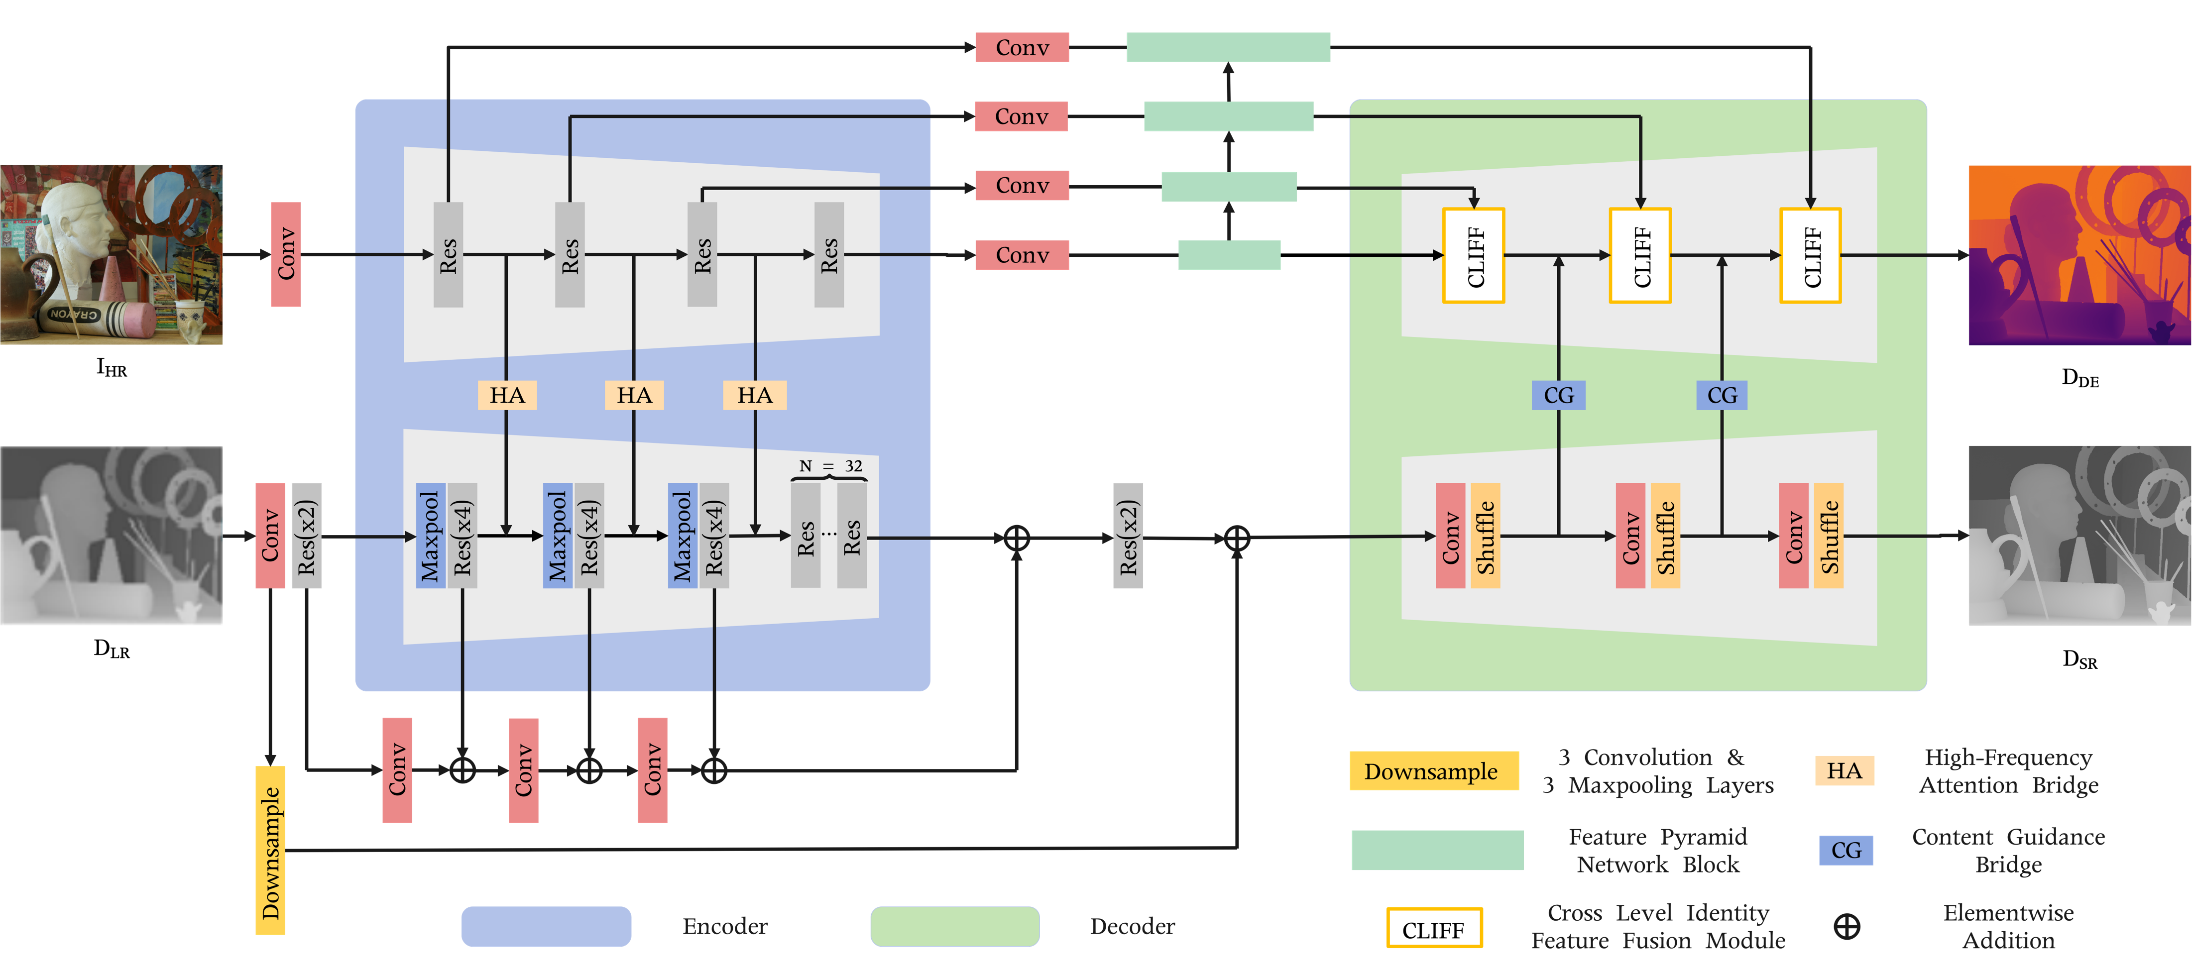
\includegraphics[scale=0.5]{14.png}};
      	\node[below = 2mm of network,shift={(0,3mm)},font={\small}]{\color{captiongray}图3 单目深度估计子网络(MDENet)};
      	\onslide<2->{
      		\draw[draw=none,fill=white,fill opacity=0.9] (0.2,6.6) rectangle(14,3.1);
      		\draw[draw=none,fill=darkgray, fill opacity=0.5] (12.6,8.6) circle(0.45);
      		\node[anchor=north east,font={\large}] at({12.9cm,8.9cm}) {\color{white}\textbf{1}};
         }
         \onslide<3-3>{
         	\draw[draw=darkred,thick,dashed] (2.2,8.8) rectangle(6.2,6.5);
         }
         \onslide<4-4>{
         	\draw[draw=darkgreen,thick,dashed] (6.2,8.8) rectangle(8.5,6.5);
         }
         \onslide<5->{
         	\draw[draw=darkblue,thick,dashed] (8.45,8.8) rectangle(11.8,6.5);
         }
         
      \end{tikzpicture}
      }
\end{frame}

\begin{frame}
\frametitle{深度图像超分辨率重建子网络}
\onslide<1->{
	\vspace{0.5cm}
    \begin{tikzpicture}
    	\useasboundingbox (0,0) rectangle(\the\paperwidth,\the\paperheight);
      	\node(network)[anchor=north east] at ({\the\paperwidth-2.5cm,\the\paperheight}) {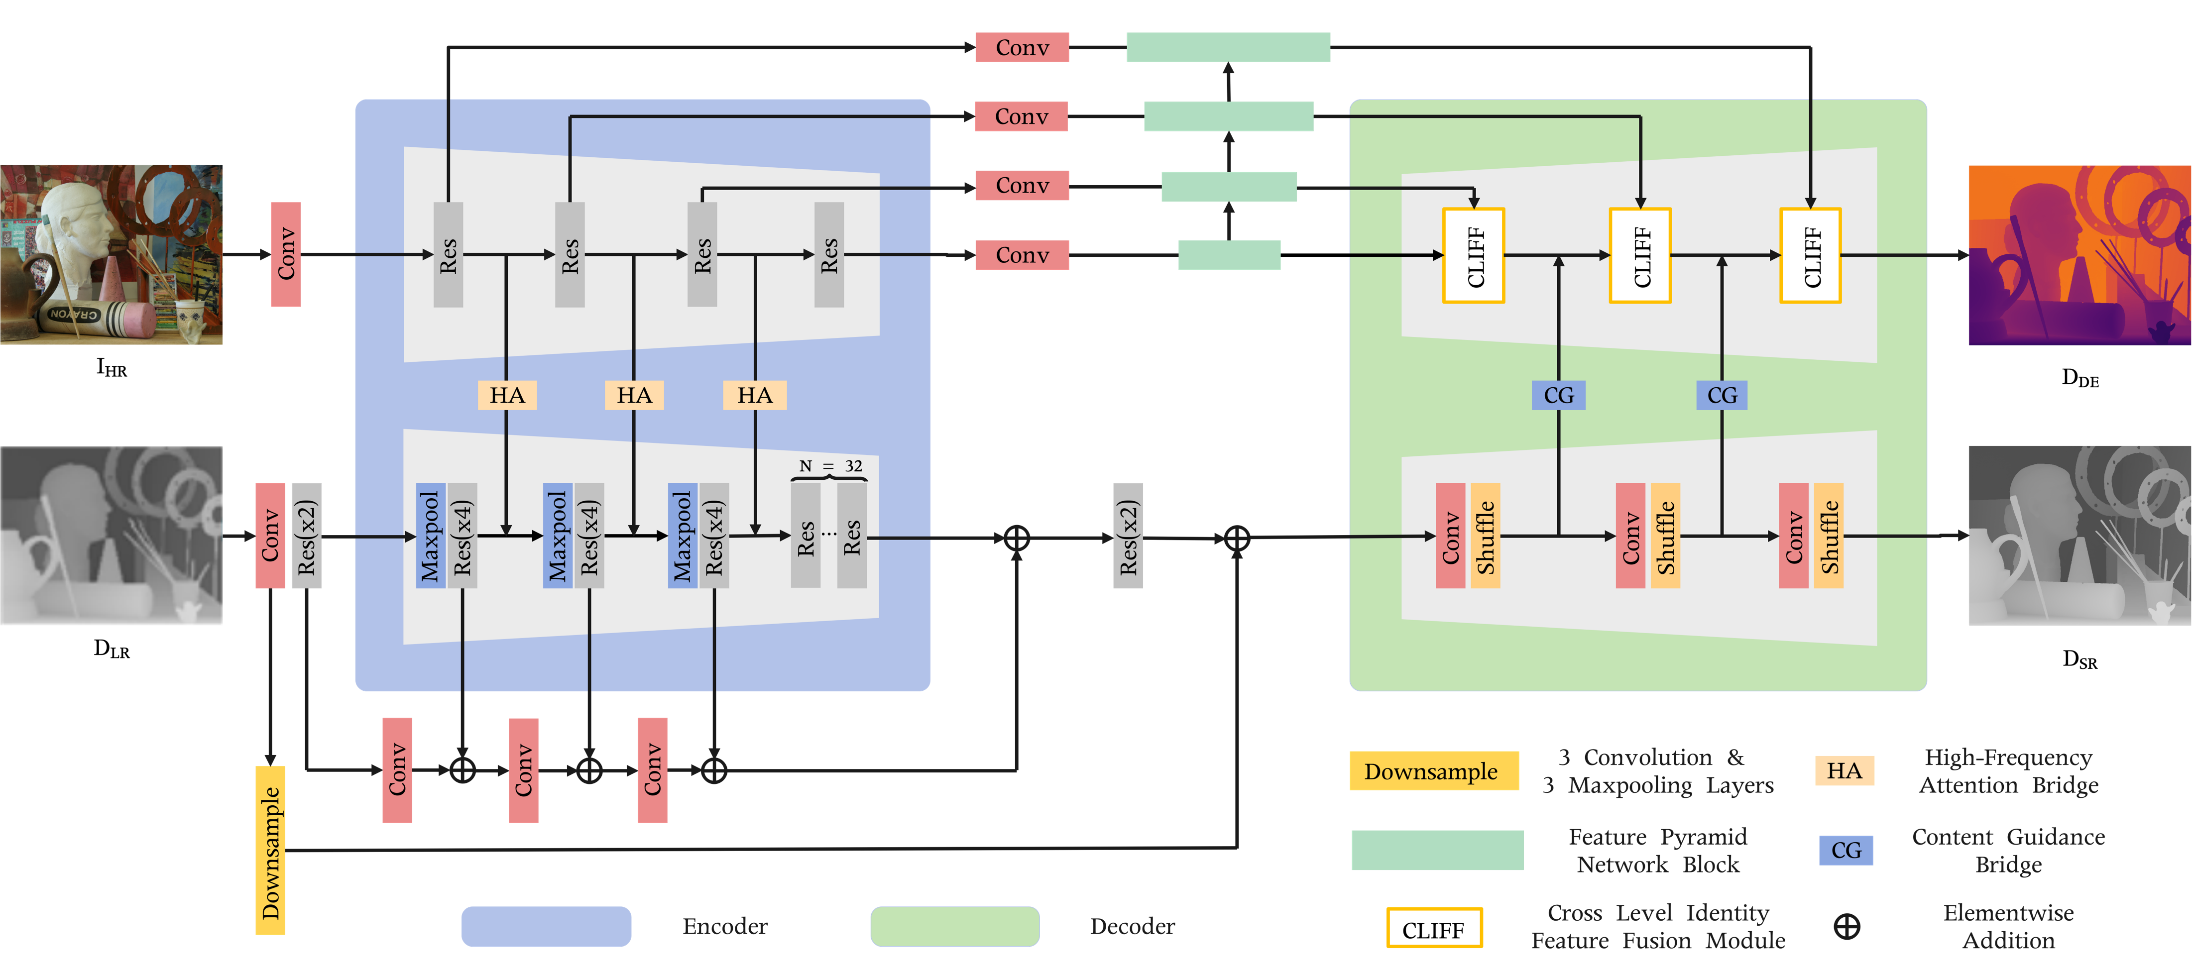
\includegraphics[scale=0.5]{14.png}};
      	\node[below = 2mm of network,shift={(0,3mm)},font={\small}]{\color{captiongray}图4 深度图像超分辨率重建子网络(DSRNet)};
      	\onslide<2->{
      		\draw[draw=none,fill=white,fill opacity=0.9] (0.2,6.6) rectangle(14,9.1);
      		\draw[draw=none,fill=darkgray, fill opacity=0.5] (1.3,4.3) circle(0.45);
      		\node[anchor=north east,font={\large}] at({1.58cm,4.6cm}) {\color{white}\textbf{2}};
         }
         \onslide<3-3>{
         	\draw[draw=darkred,thick,dashed] (2.1,6.5) rectangle(5,5);
         }
         \onslide<4-4>{
         	\draw[draw=darkgreen,thick,dashed] (5,6.5) rectangle(6,5);
         }
         \onslide<5-5>{
         	\draw[draw=darkblue,thick,dashed] (2.6,4.8) rectangle(6,3.8);
         }
         \onslide<6-6>{
         	\draw[draw=darkred,thick,dashed] (8.45,6.5) rectangle(11.8,5);
         }
         \onslide<7-7>{
         	\draw[draw=darkgreen,thick,dashed] (7.5,6.5) rectangle(8.2,5);
         }
         \onslide<8-8>{
         	\draw[draw=darkblue,thick,dashed] (1.9,3.2) rectangle(2.6,4.7);
         }
      \end{tikzpicture}
      }
	
\end{frame}

\begin{frame}[t]
\frametitle{高频注意力桥}	
	\onslide<1-1>{
		\vspace{0.5cm}
		\begin{figure}
			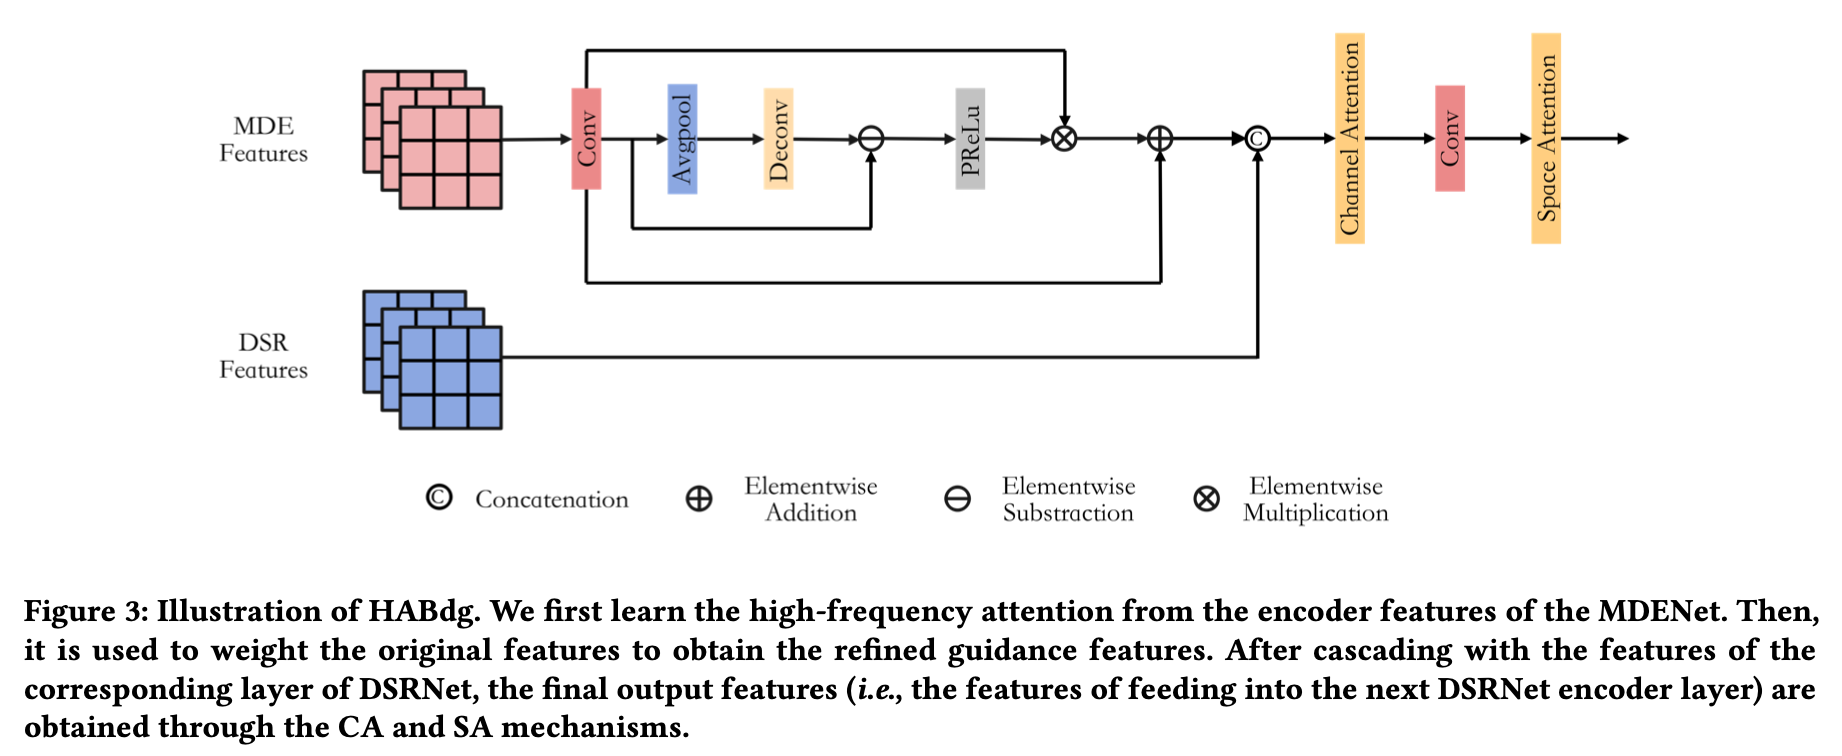
\includegraphics[scale=0.35]{16.png}
			\caption{\small\color{captiongray}图5 高频注意力桥(HABdg)}
		\end{figure}
	}
	\onslide<2->{
		\vspace{-6.7cm}
		\begin{columns}
			\begin{column}{0.5\linewidth}
				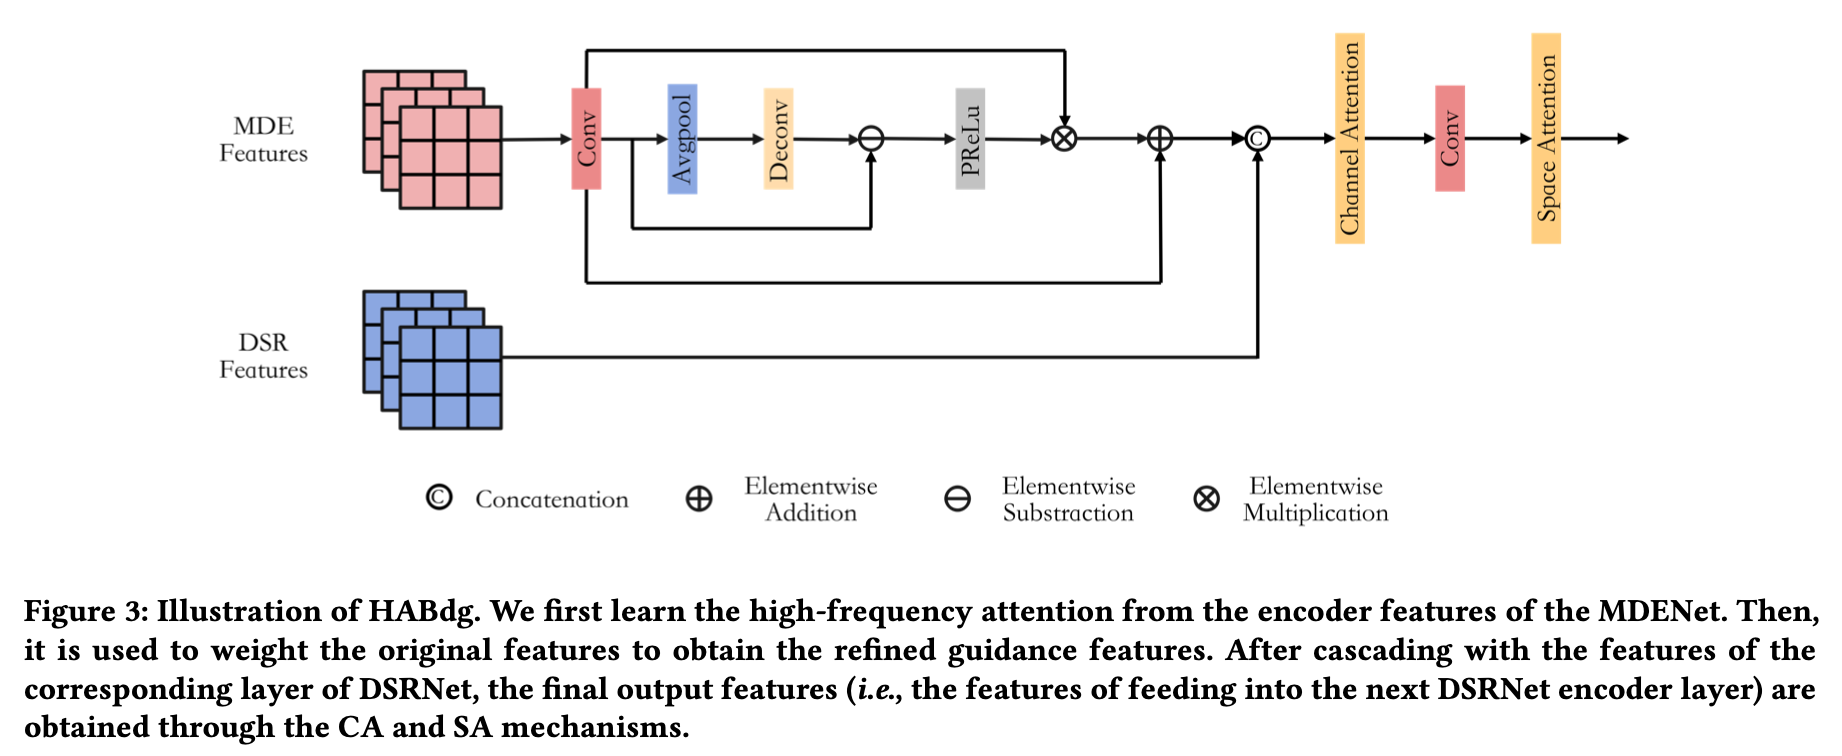
\includegraphics[scale=0.26]{16.png}
			\end{column}
			\begin{column}{0.5\linewidth}
				\begin{equation}
					\footnotesize
					\begin{gathered}
						F_{\text {blurred }}^{i}=\operatorname{deconv}\left(\operatorname{avgpool}\left(F_{M D E}^{i}\right)\right) \\
						A_{h f}^{i}=\operatorname{Pelu}\left(F_{M D E}^{i}-F_{\text {blurred }}^{i}\right) \\
						F_{h g}^{i}=F_{M D E}^{i}+A_{h f}^{i} \cdot F_{M D E}^{i} \\
						F_{\text {comp }}^{i}=\left[F_{D S R}^{i}, F_{h g}^{i}\right] \\
						F_{h a}^{i}=S A\left(\operatorname{conv}_{1 \times 1}\left(\operatorname{CA}\left(F_{\text {comp }}^{i}\right)\right)\right)
					\end{gathered}
				\end{equation}	
			\end{column}

		\end{columns}
		
		\footnotesize
		$F_{M D E}^{i}, F_{\text {blurred }}^{i}$ —— 单目深度估计子网络第 $i$ 层的特征和获得的模糊特征;\\
		$A_{h f}^{i}, F_{h g}^{i}-$ —— 获得的第 $i$ 层的高频注意力和优化后的引导特征;\\
		$F_{D S R}^{i}, F_{h a}^{i}$ —— 深度图像超分辨率重建子网络第 $i$ 层的特征和融合高频信息的特征;\\
		$\operatorname{avgpool}(\cdot)$  —— 平均池化操作; $\operatorname{deconv}(\cdot)$  —— 反卷积操作; $\operatorname{con}_{1 \times 1}$ —— 卷积核大小为 $1 \times 1$ 的卷积层;\\
		$P \operatorname{Relu}(\cdot)$ —— 带参数的修正线性单元,即激活函数;\\
		$CA, SA$ —— 通道注意力,空间注意力; $[\cdot,\cdot]$ —— 通道维度的级联。
	}
\end{frame}

\begin{frame}[t]
\frametitle{内容引导桥}	
	\onslide<1-1>{
		\begin{columns}
			\begin{column}{0.6\textwidth}
				\begin{figure}
					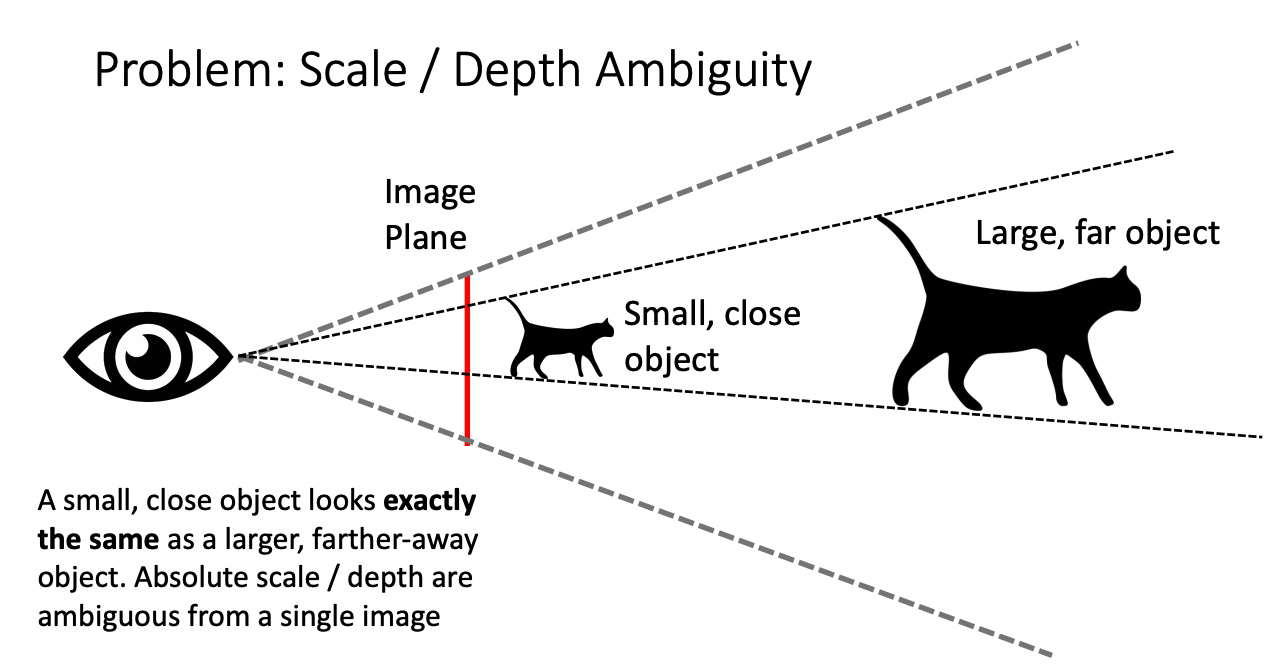
\includegraphics[scale=0.18]{17.png}
					\caption{\small\color{captiongray}图6 尺度模糊性}
				\end{figure}
			\end{column}
			\begin{column}{0.4\textwidth}
				\begin{figure}
					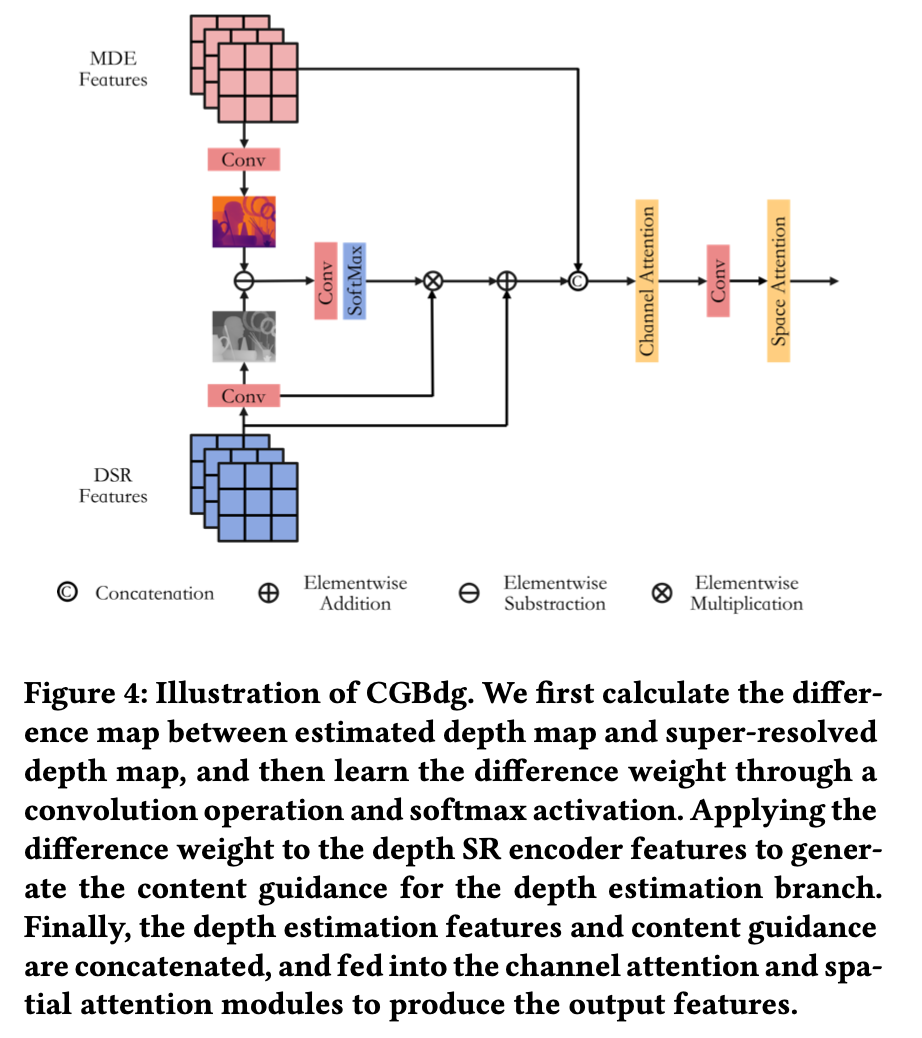
\includegraphics[scale=0.3]{18.png}
					\caption{\small\color{captiongray}图7 内容引导桥(CGBdg)}
				\end{figure}
			\end{column}

	
		\end{columns}
	}
	\onslide<2->{
		\vspace{-6.5cm}
		\begin{columns}
			\begin{column}{0.4\textwidth}	
				\begin{figure}
					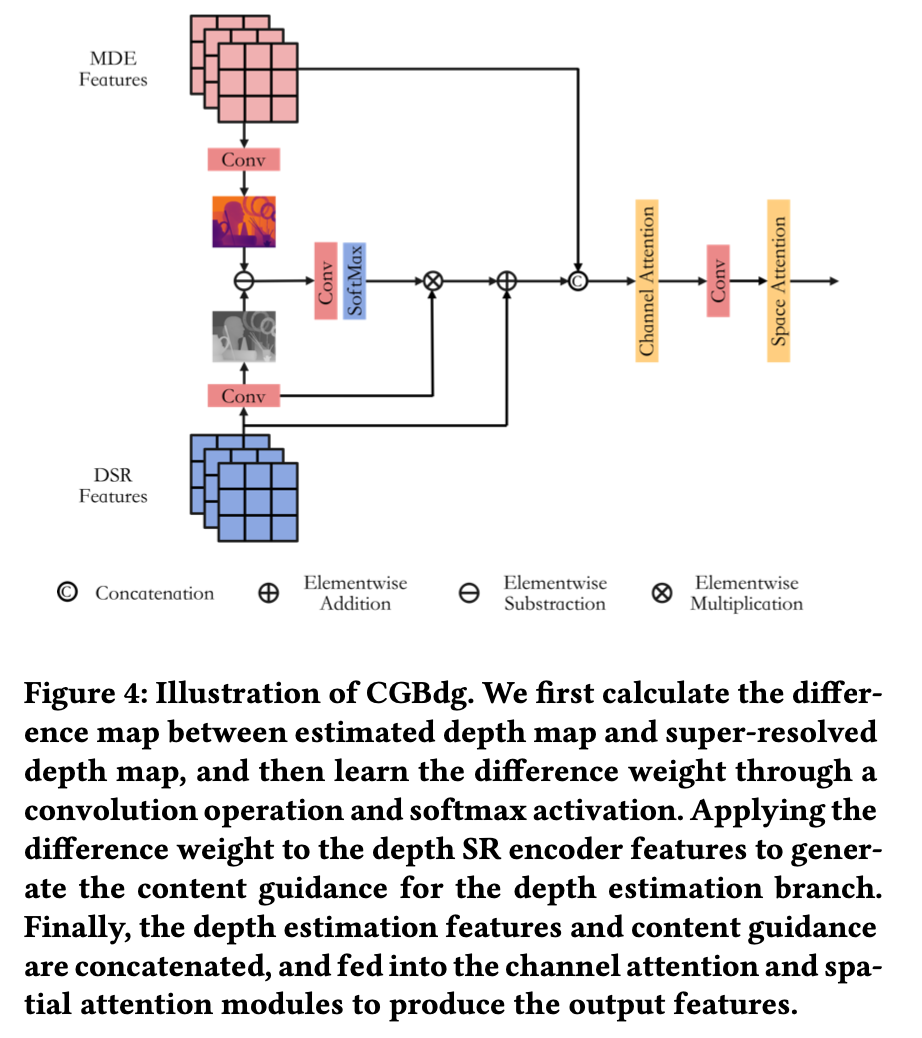
\includegraphics[scale=0.3]{18.png}
				\end{figure}
			\end{column}
			\begin{column}{0.6\textwidth}	
				\footnotesize
				\begin{equation}
					\begin{gathered}
						M_{D S R}^{i}=\operatorname{conv}_{1 \times 1}\left(F d_{D S R}^{i}\right) \\
						M_{M D E}^{i}=\operatorname{conv}_{1 \times 1}\left(F d_{M D E}^{i}\right) \\
						W_{d i f f}^{i}=\operatorname{softmax}\left(\operatorname{conv}_{1 \times 1}\left(M_{D S R}^{i}-M_{M D E}^{i}\right)\right) \\
						F_{c g}^{i}=F d_{D S R}^{i}+W_{d i f f}^{i} * F d_{D S R}^{i}
					\end{gathered}
				\end{equation}
				
				$M_{D S R}^{i}$ —— 深度图像超分辨率重建子网络第 $i$ 层生成的深度图像;\\[0.2em]
				$M_{M D E}^{i}$ —— 单目深度估计子网络第 $i$ 层估计的深度图像;\\[0.2em]   
				$F d_{D S R}^{i}$ —— 深度图像超分辨率重建子网络解码器第 $i$ 层的特征;\\[0.2em]
				$F d_{M D E}^{i}$ —— 单目深度估计子网络解码器第 $i$ 层的特征。\\[0.2em]
				$W_{\text {diff }}^{i}$ —— 差异权重;\\[0.2em]
				$F_{c g}^{i}$ —— 第 $i$ 层的内容引导特征。

			\end{column}

		\end{columns}

	}
\end{frame}

\begin{frame}[t]
\frametitle{联合学习策略}	
	\begin{columns}
		\begin{column}{0.35\textwidth}
			\begin{figure}
				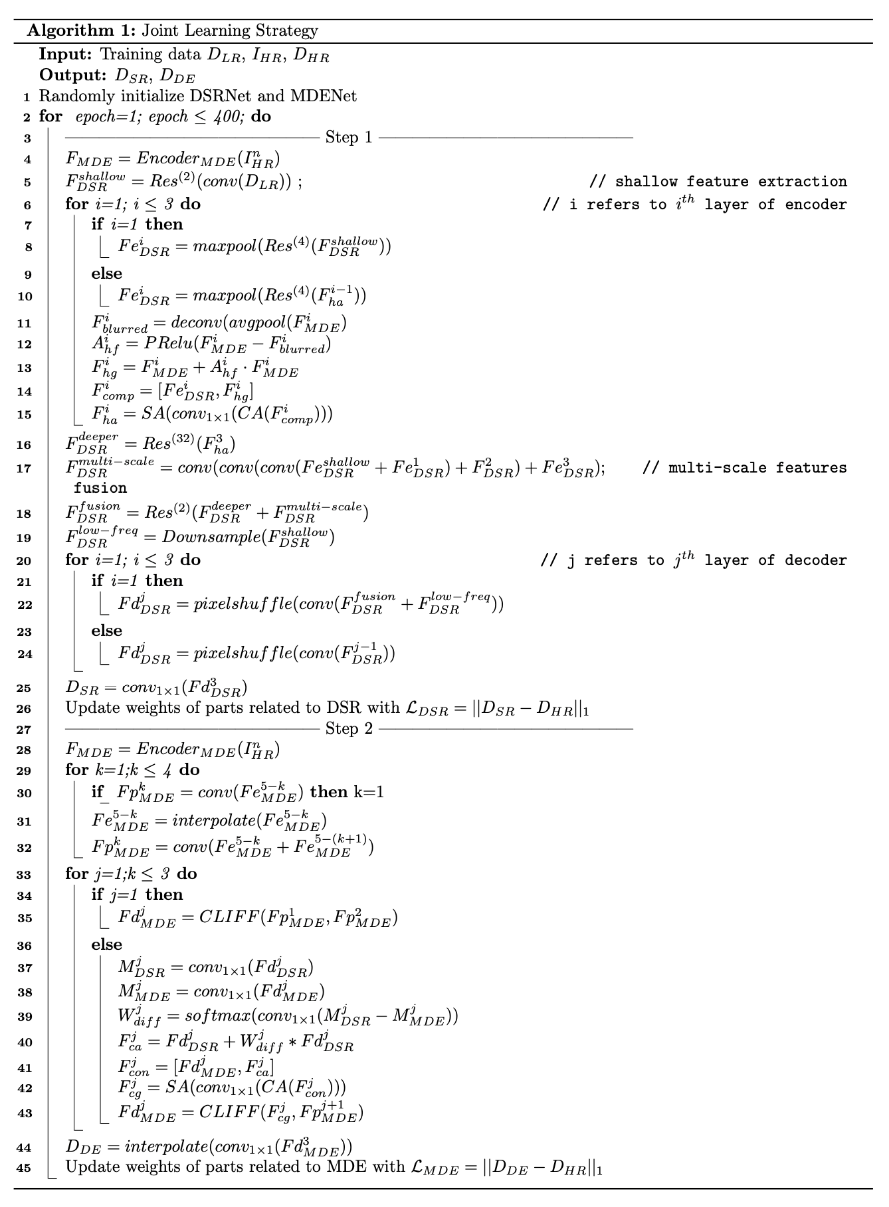
\includegraphics[scale=0.45]{19.png}
			\end{figure}
		\end{column}
		\begin{column}{0.65\textwidth}
		\small
		本文分别为深度图像超分辨率重建和单目深度估计的损失函数分配了不同的优化器。这是因为深度图像超分辨率重建和单目深度估计的学习难度大不相同,导致两个任务的收敛速度不同,从而很难找到合适的权重设置来确保两个任务都达到最佳性能。因此,在损失函数的设计方面,本文提出分别对深度图像超分辨率重建和单目深度估计相关部分进行优化的策略。其损失函数定义为
		
		{\footnotesize
		\begin{equation}
			\begin{aligned}
				&\mathcal{L}_{D S R}=\left\|D_{S R}-D_{H R}\right\|_{1} \\
				&\mathcal{L}_{M D E}=\left\|D_{D E}-D_{H R}\right\|_{1}
			\end{aligned}
		\end{equation}

		$\mathcal{L}_{D S R}$ —— 深度图像超分辨率重建任务的逐像素 $L_1$ 损失;\\
		$\mathcal{L}_{D S R}$ —— 单目深度估计任务的逐像素 $L_1$ 损失。}

			
		\end{column}
	\end{columns}

\end{frame}

\section{研究成果}
\subsection{实现细节}
\begin{frame}[t]
	\frametitle{实现细节}
	\begin{columns}
		\begin{column}{0.45\textwidth}
			\begin{figure}
				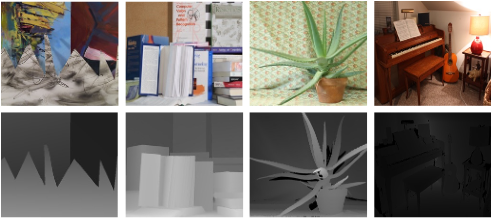
\includegraphics[height=2.5cm]{20.png}
			\end{figure}
			\begin{equation}
				\scriptsize
				M A D_{\text {Middlebury }}=\frac{1}{N} \sum_{n=1}^{N}\left|D_{H R}^{n}-S R\left(D_{L R}^{n}\right)\right|
			\end{equation}		
		\end{column}
		\begin{column}{0.45\textwidth}
			\begin{figure}
				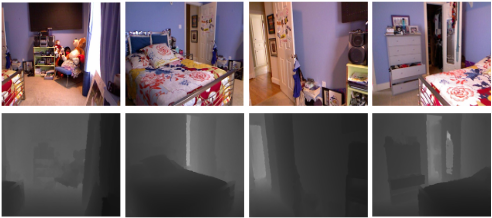
\includegraphics[height=2.5cm]{21.png}
			\end{figure}
			\begin{equation}
				\scriptsize
				R M S E_{N Y U v 2}=\sqrt{\frac{1}{M} \sum_{m=1}^{M}\left(D_{H R}^{m}-S R\left(D_{L R}^{m}\right)\right)^{2}}
			\end{equation}	
			
		\end{column}
	
	\end{columns}
	\footnotesize 高分辨率的深度图像和彩色图像分别根据 $\times4$ 、$\times 8$ 和 $\times 16$ 的上采样因子被裁剪成足够数量的大小为 $64^2$、$128^2$ 和 $256^2$ 的图像块。为了获得相应的低分辨率深度图像块,使用 Bicubic 插值方法将高分辨率深度图像块下采样为固定大小的 $16 \times 16$ 的图像块。
	
	网络基于 PyTorch 实现,并使用 NVIDIA 2080Ti GPU 加速训练。在训练期间,一次训练所选取的样本数为8 。此外,选取了动量为 0.9,$\beta_1=0.9$,$\beta_2=0.99$,$\epsilon=10^{−8}$ 的 ADAM 优化器对训练进行优化。初始学习率设置为 $1𝑒^{−4}$ ,并且每100轮乘以0.1以降低学习速率。
\end{frame}

\subsection{实验结果}
\begin{frame}[t]
	\frametitle{实验结果}
	\begin{figure}
		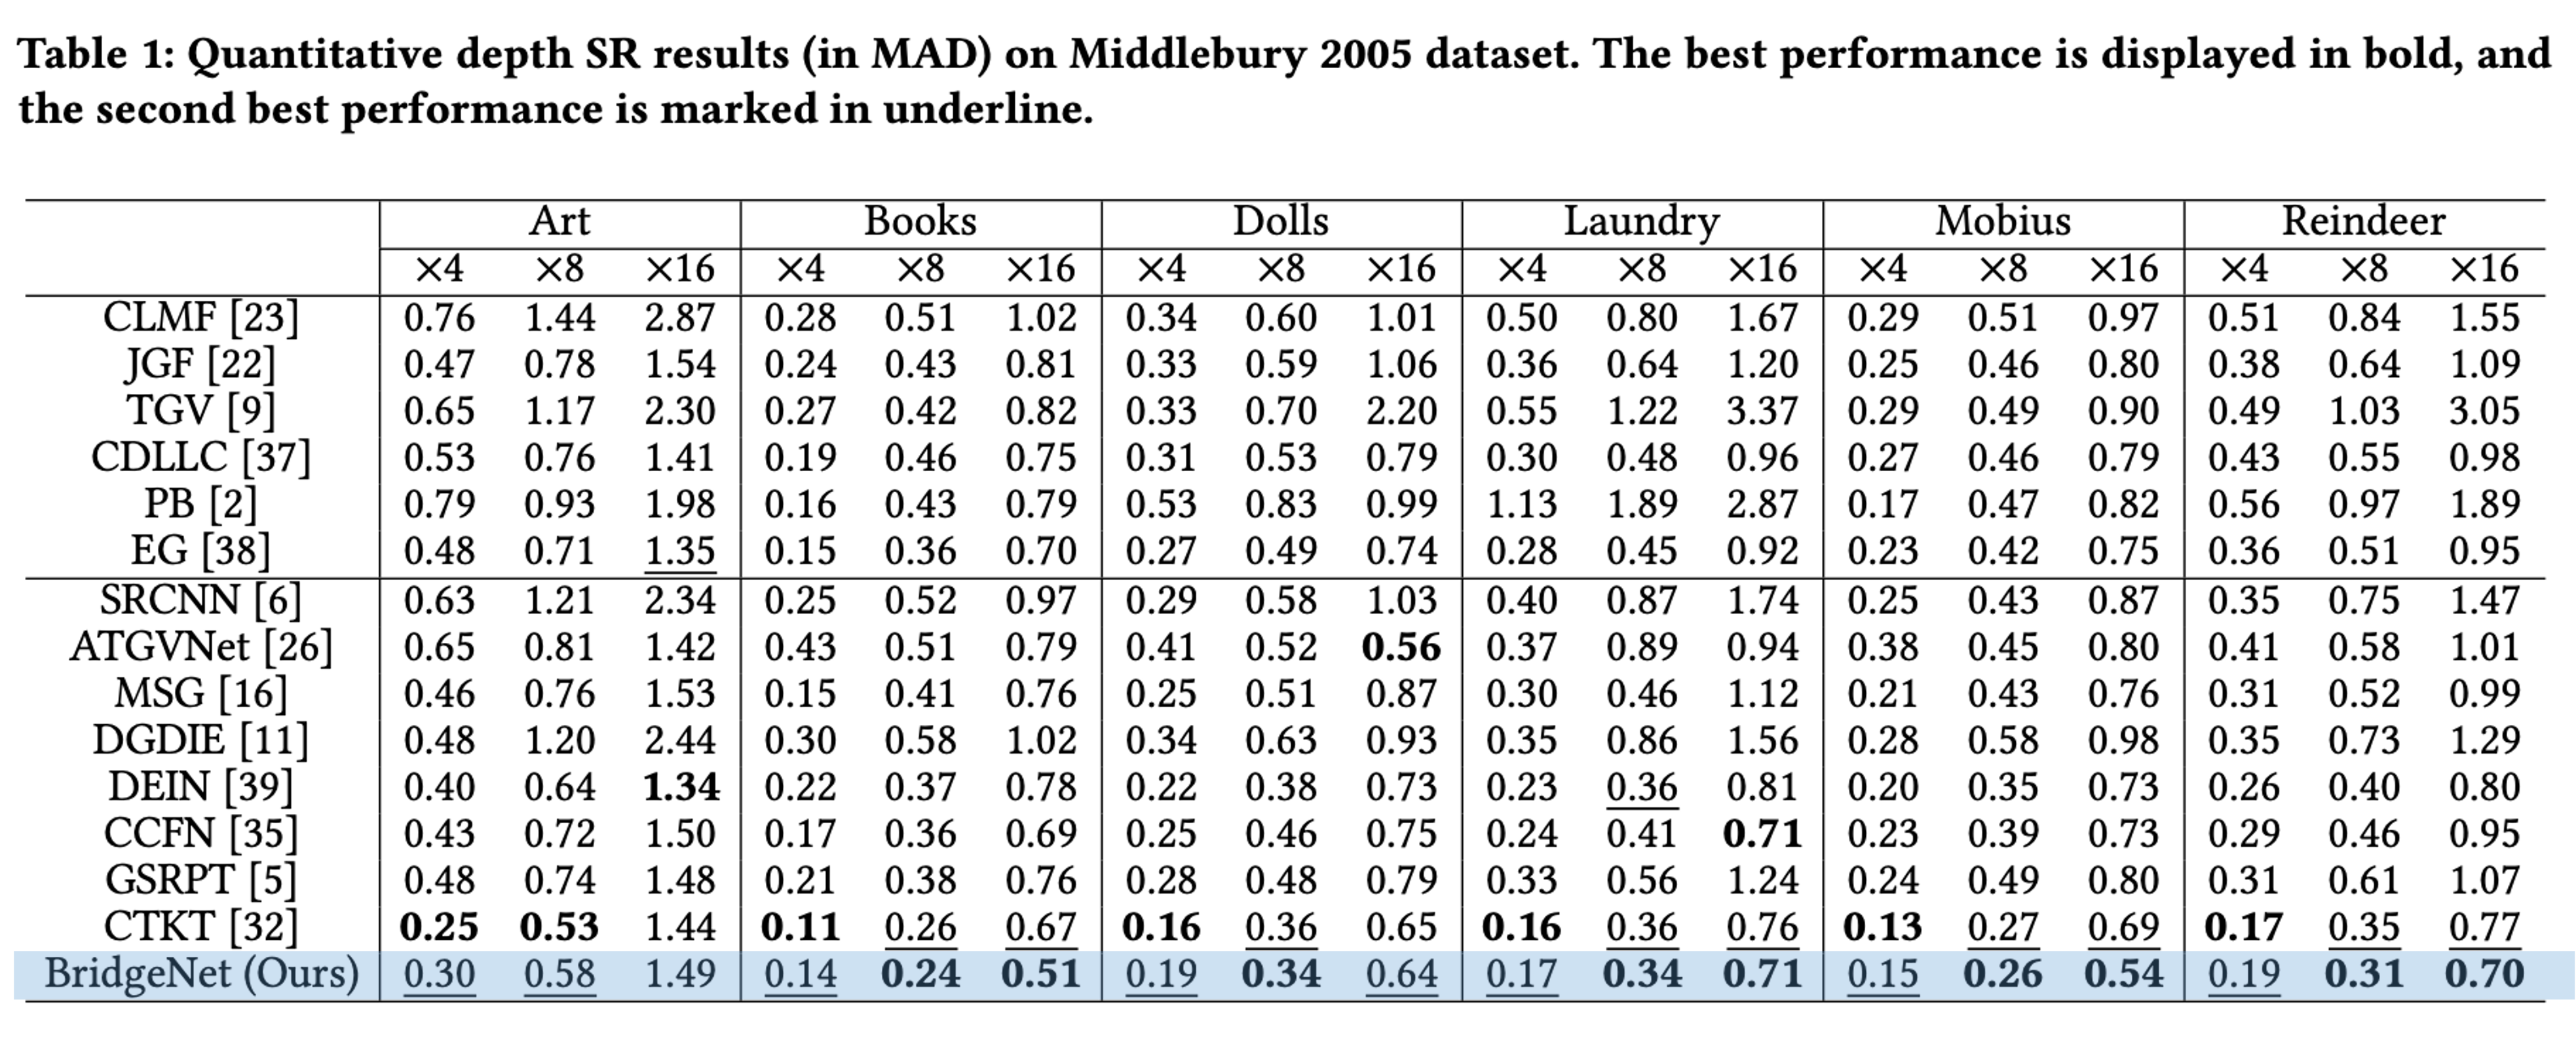
\includegraphics[scale=0.45]{22.png}
	\end{figure}
\end{frame}

\begin{frame}[t]
	\frametitle{实验结果}
	\begin{figure}
		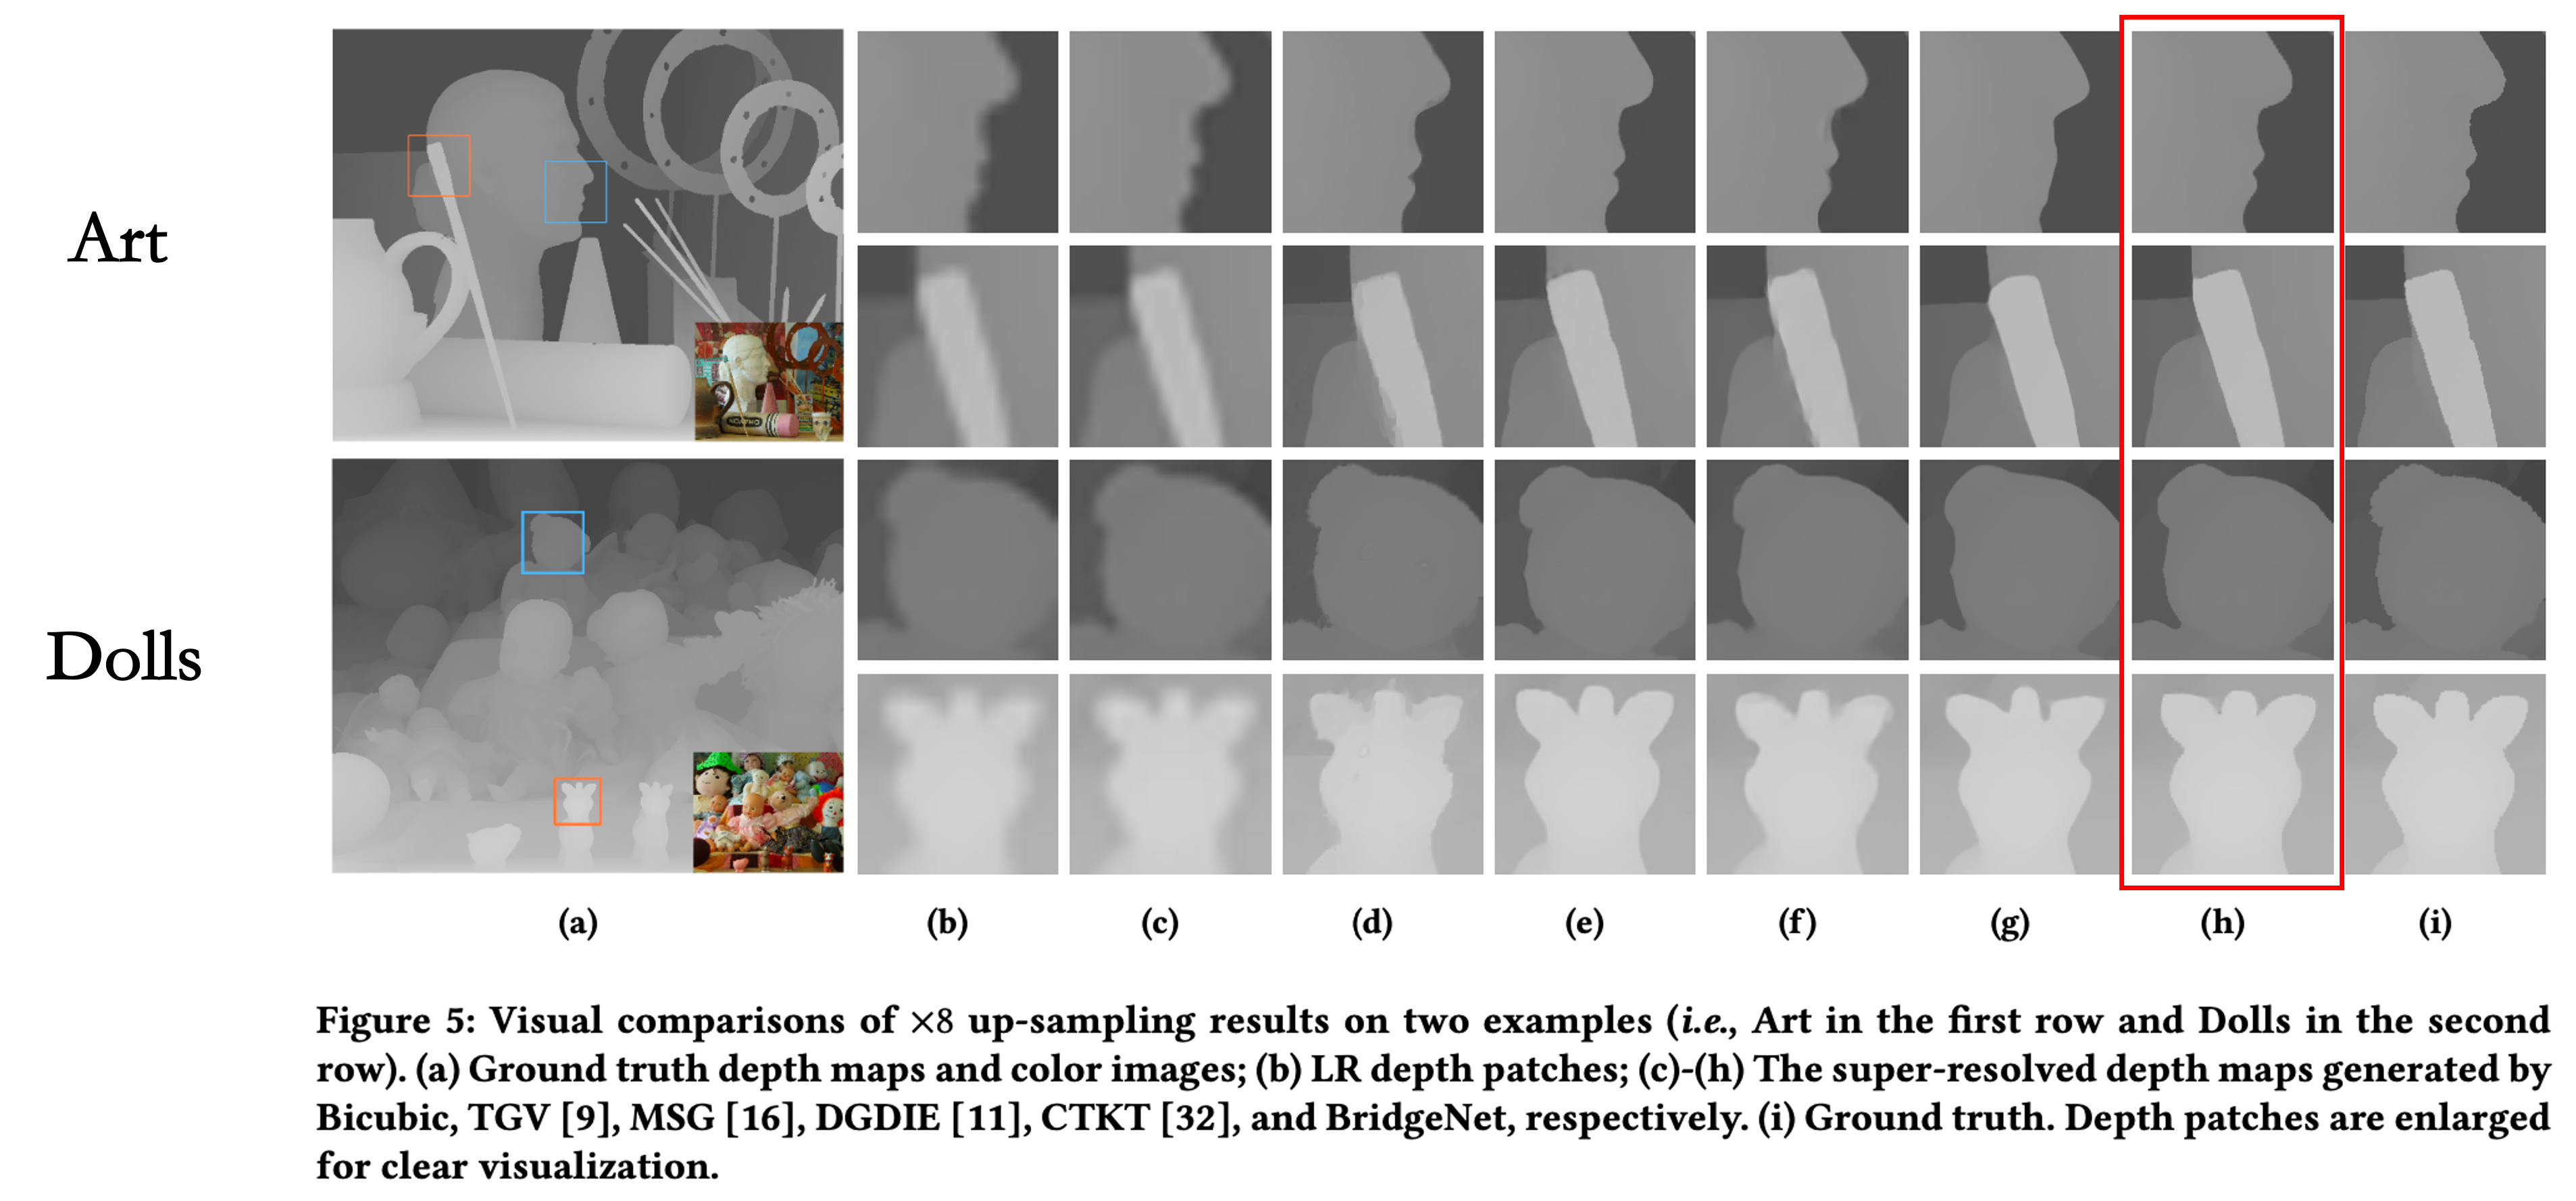
\includegraphics[scale=0.45]{23.png}
	\end{figure}
\end{frame}

\subsection{消融实验}
\begin{frame}
	\frametitle{消融实验}
	\begin{figure}
		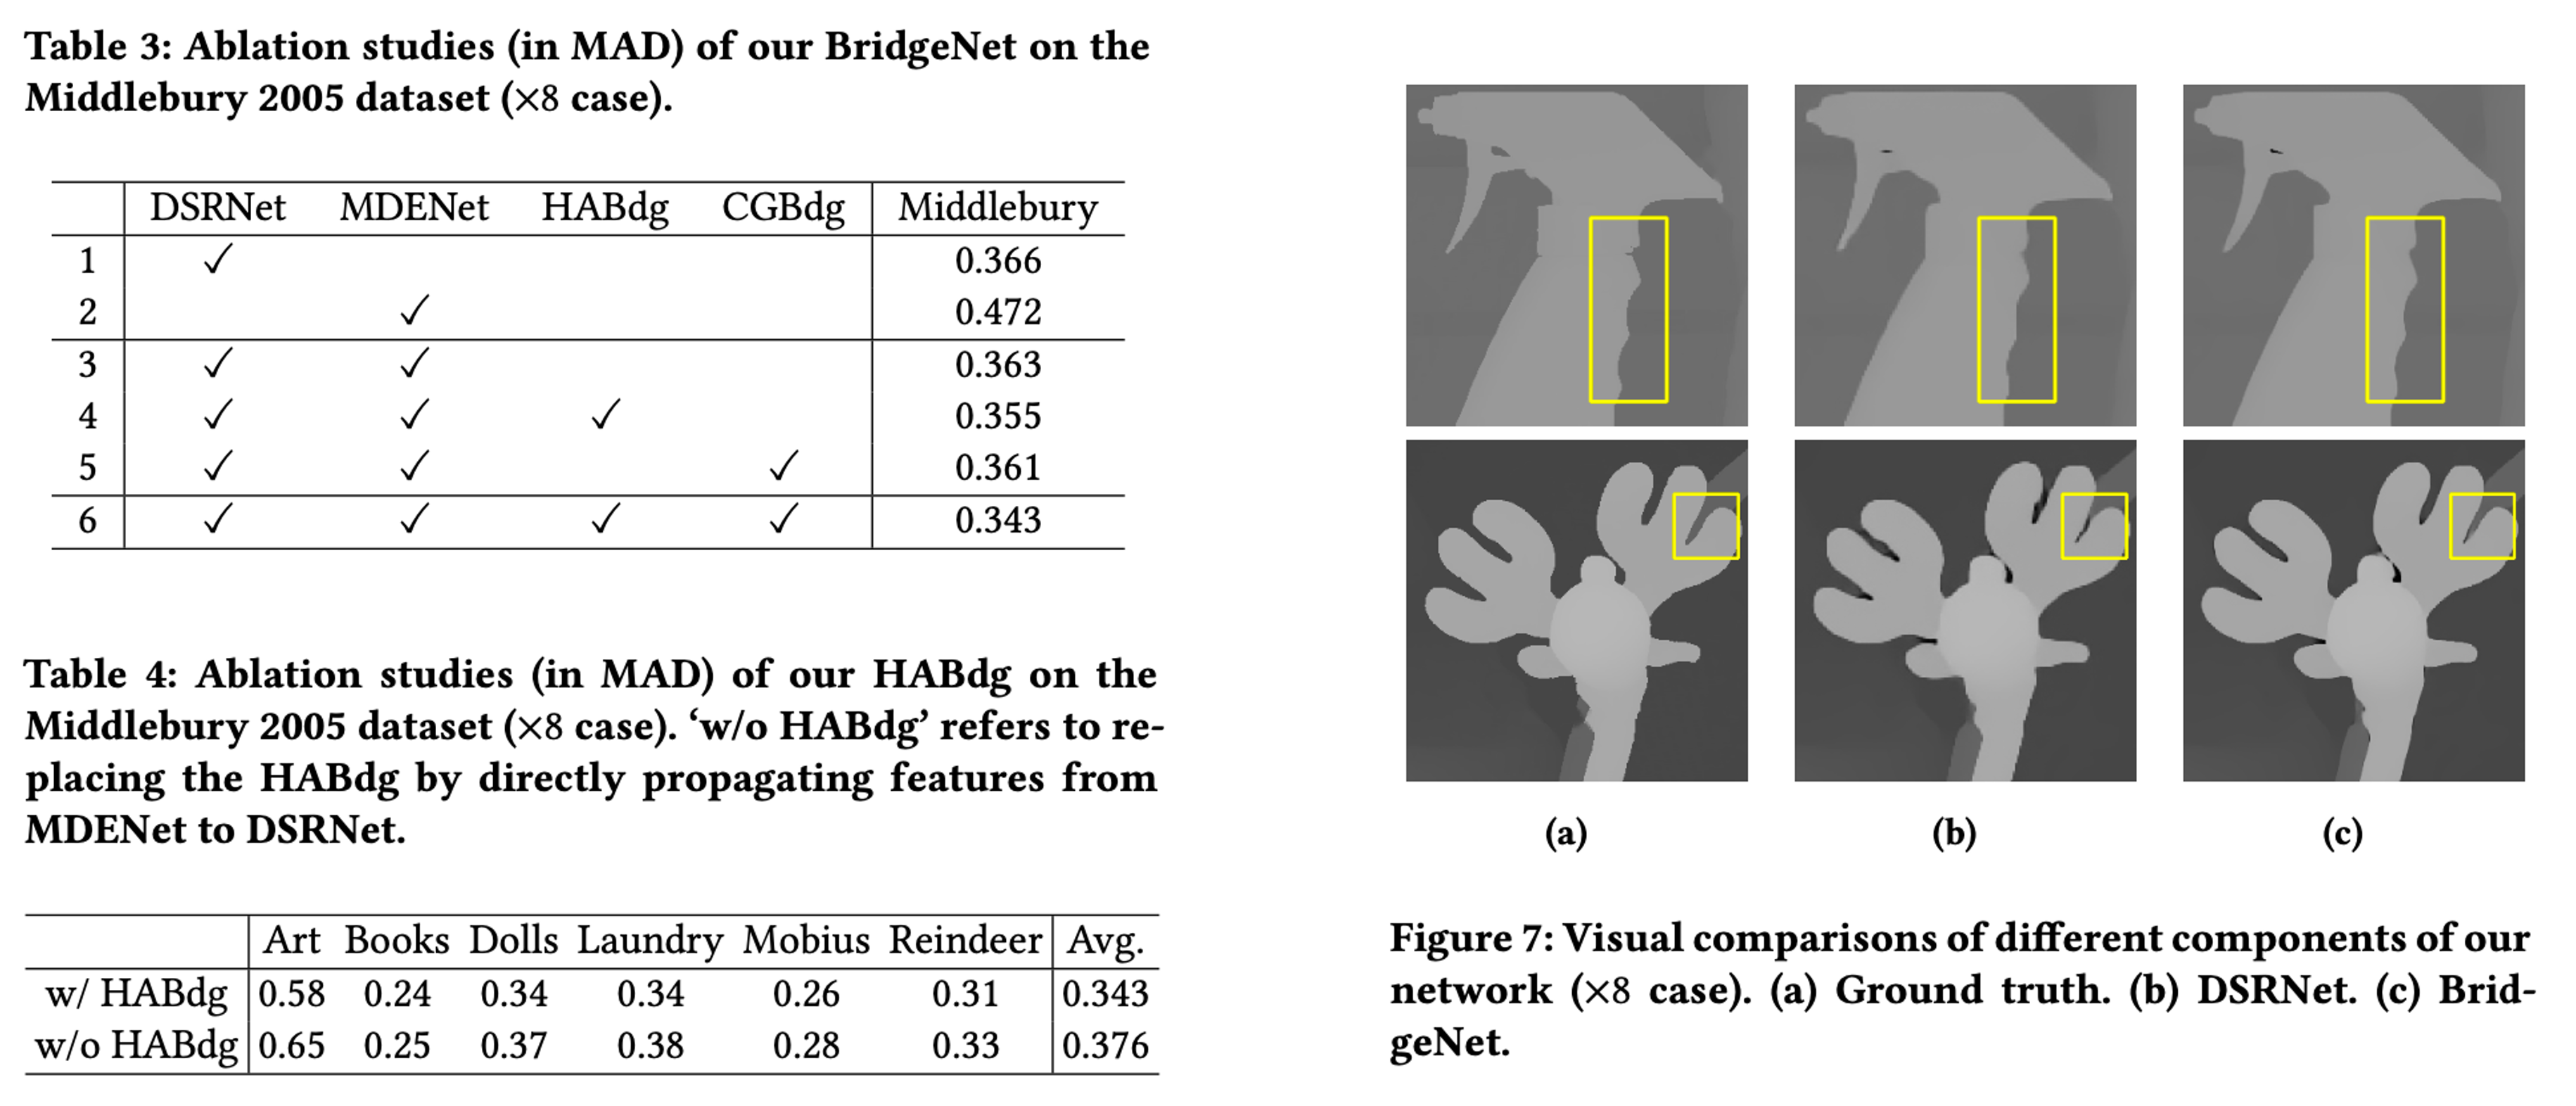
\includegraphics[scale=0.45]{24.png}
	\end{figure}
\end{frame}

\section{项目总结}
\subsection{总结归纳}
\begin{frame}[t]
	\hspace*{-0.4cm}\begin{tikzpicture}
		\draw[draw=none,fill=bjtublue] (-2,4.5) rectangle(5.3,5.1);
		\node(blocktitle)[anchor=north west,font={\normalsize}] at({0.3,5.15}) {\color{white}论文及专利};
		\draw[draw=bjtublue,thick,dotted] (-2,4.45) rectangle(5.3,1.2);
		\node(blockbody)[below=2mm of blocktitle,font={\footnotesize},align=left] {
			\begin{varwidth}{0.5\linewidth}\begin{itemize}
        		\item 发明专利:《一种联合单目深度估计的深度图像超分辨率重建方法》
        		\item 2021 ACM MM(CCF A):BridgeNet: A Joint Learning Network of Depth Map Super-Resolution and Monocular Depth Estimation
    		\end{itemize}\end{varwidth}
		};
		\node[below=1mm of blockbody,shift={(-1.6cm,0)}] {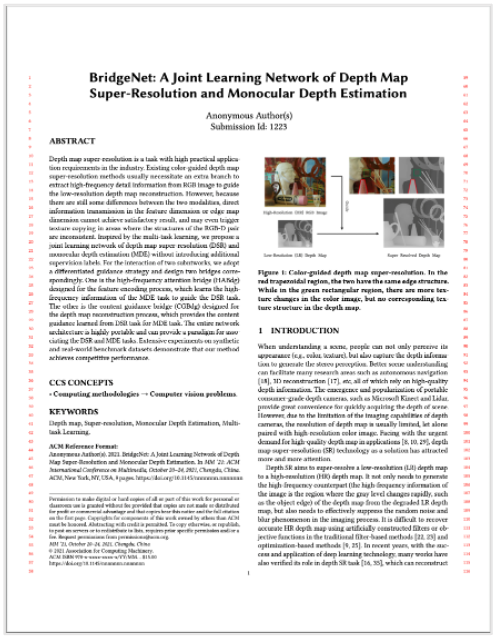
\includegraphics[scale=0.44]{25.png}};
		\node[below=1mm of blockbody,shift={(1.6cm,0)}] {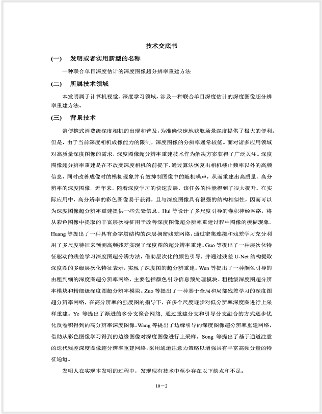
\includegraphics[scale=0.44]{26.png}};
		
		\node[right=3cm of blocktitle,shift={(0,-3.2cm)}]{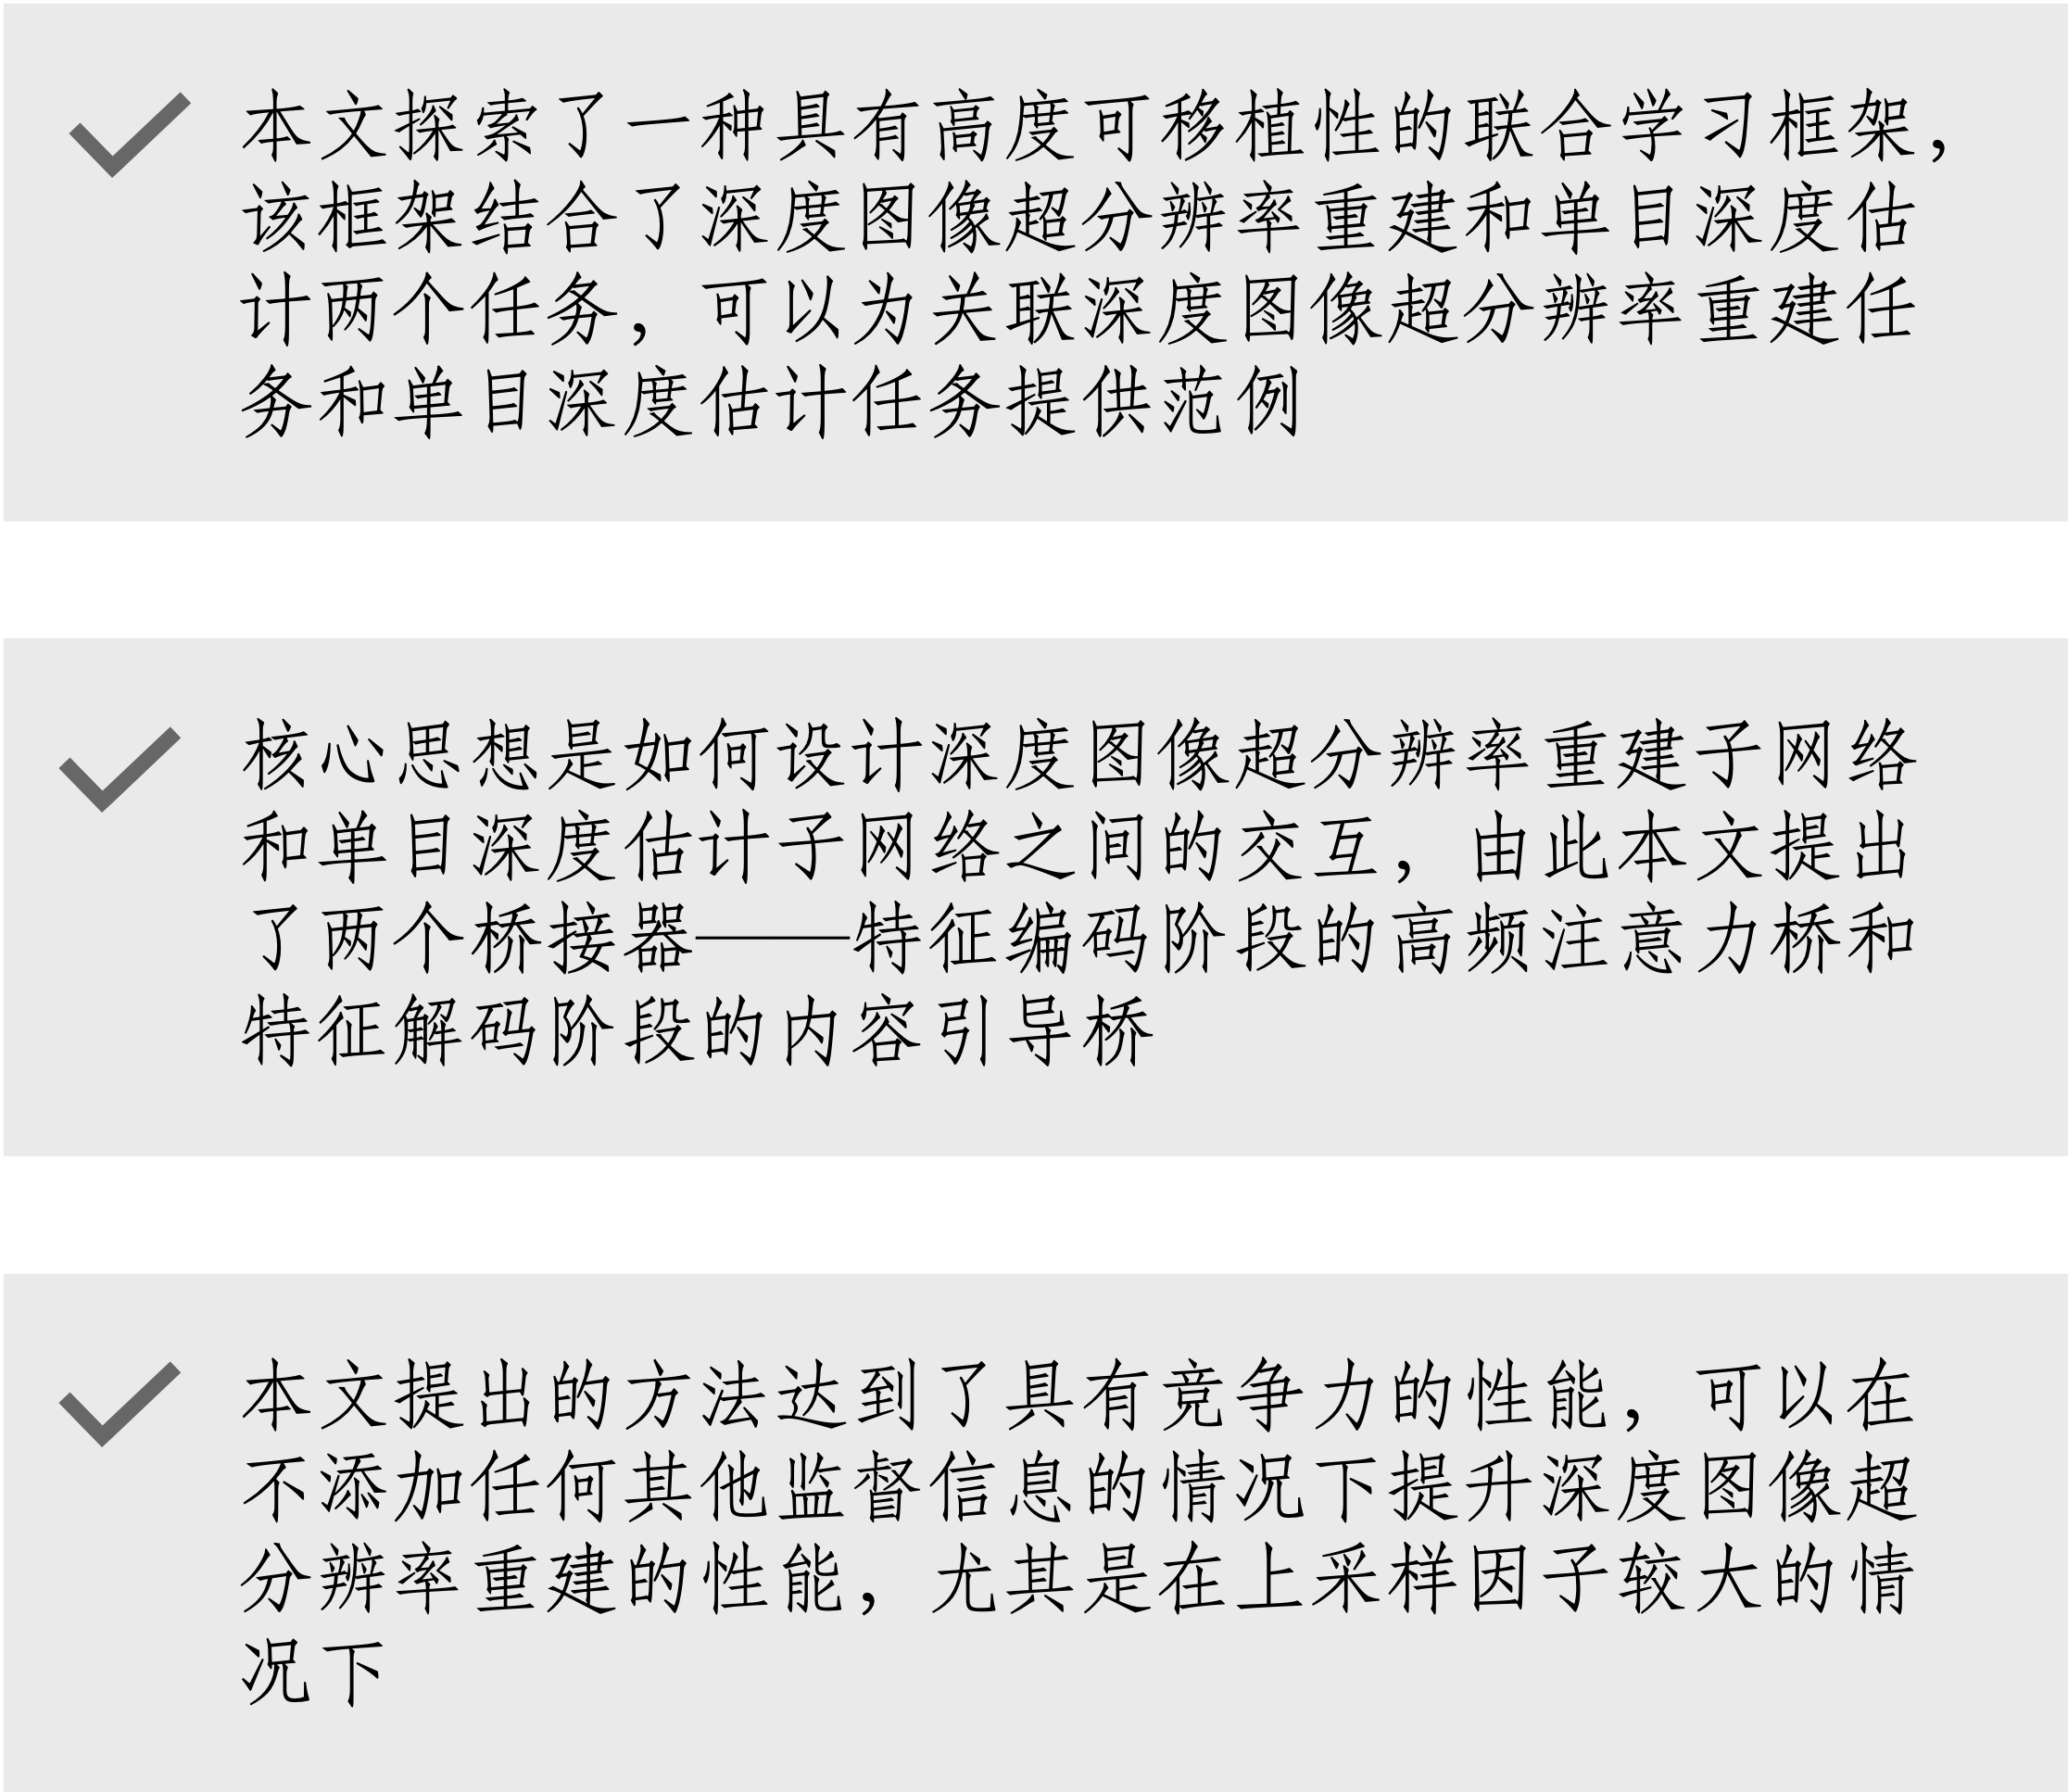
\includegraphics[scale=0.4]{27.png}};
		
	\end{tikzpicture}
\end{frame}

\makebackcover
\end{document}
